\documentclass[../SustainableHEP.tex]{subfiles}
\begin{document}
\RaggedRight
\sloppy
\newpage

%%%%%%%%%%%%%%%%%%%%%%%%%%%%%%%%%%%%%%%%

\section{Resources and Waste}
\label{sec:Waste}
%\textbf{Contributors:} Viraf Mehta, Karolos Potamianos, Enrico Cennini\\

%%%%%%%%%%%%%%%%%%%%%%%%%%%%%%%%%%%%%%%%

\begin{center}
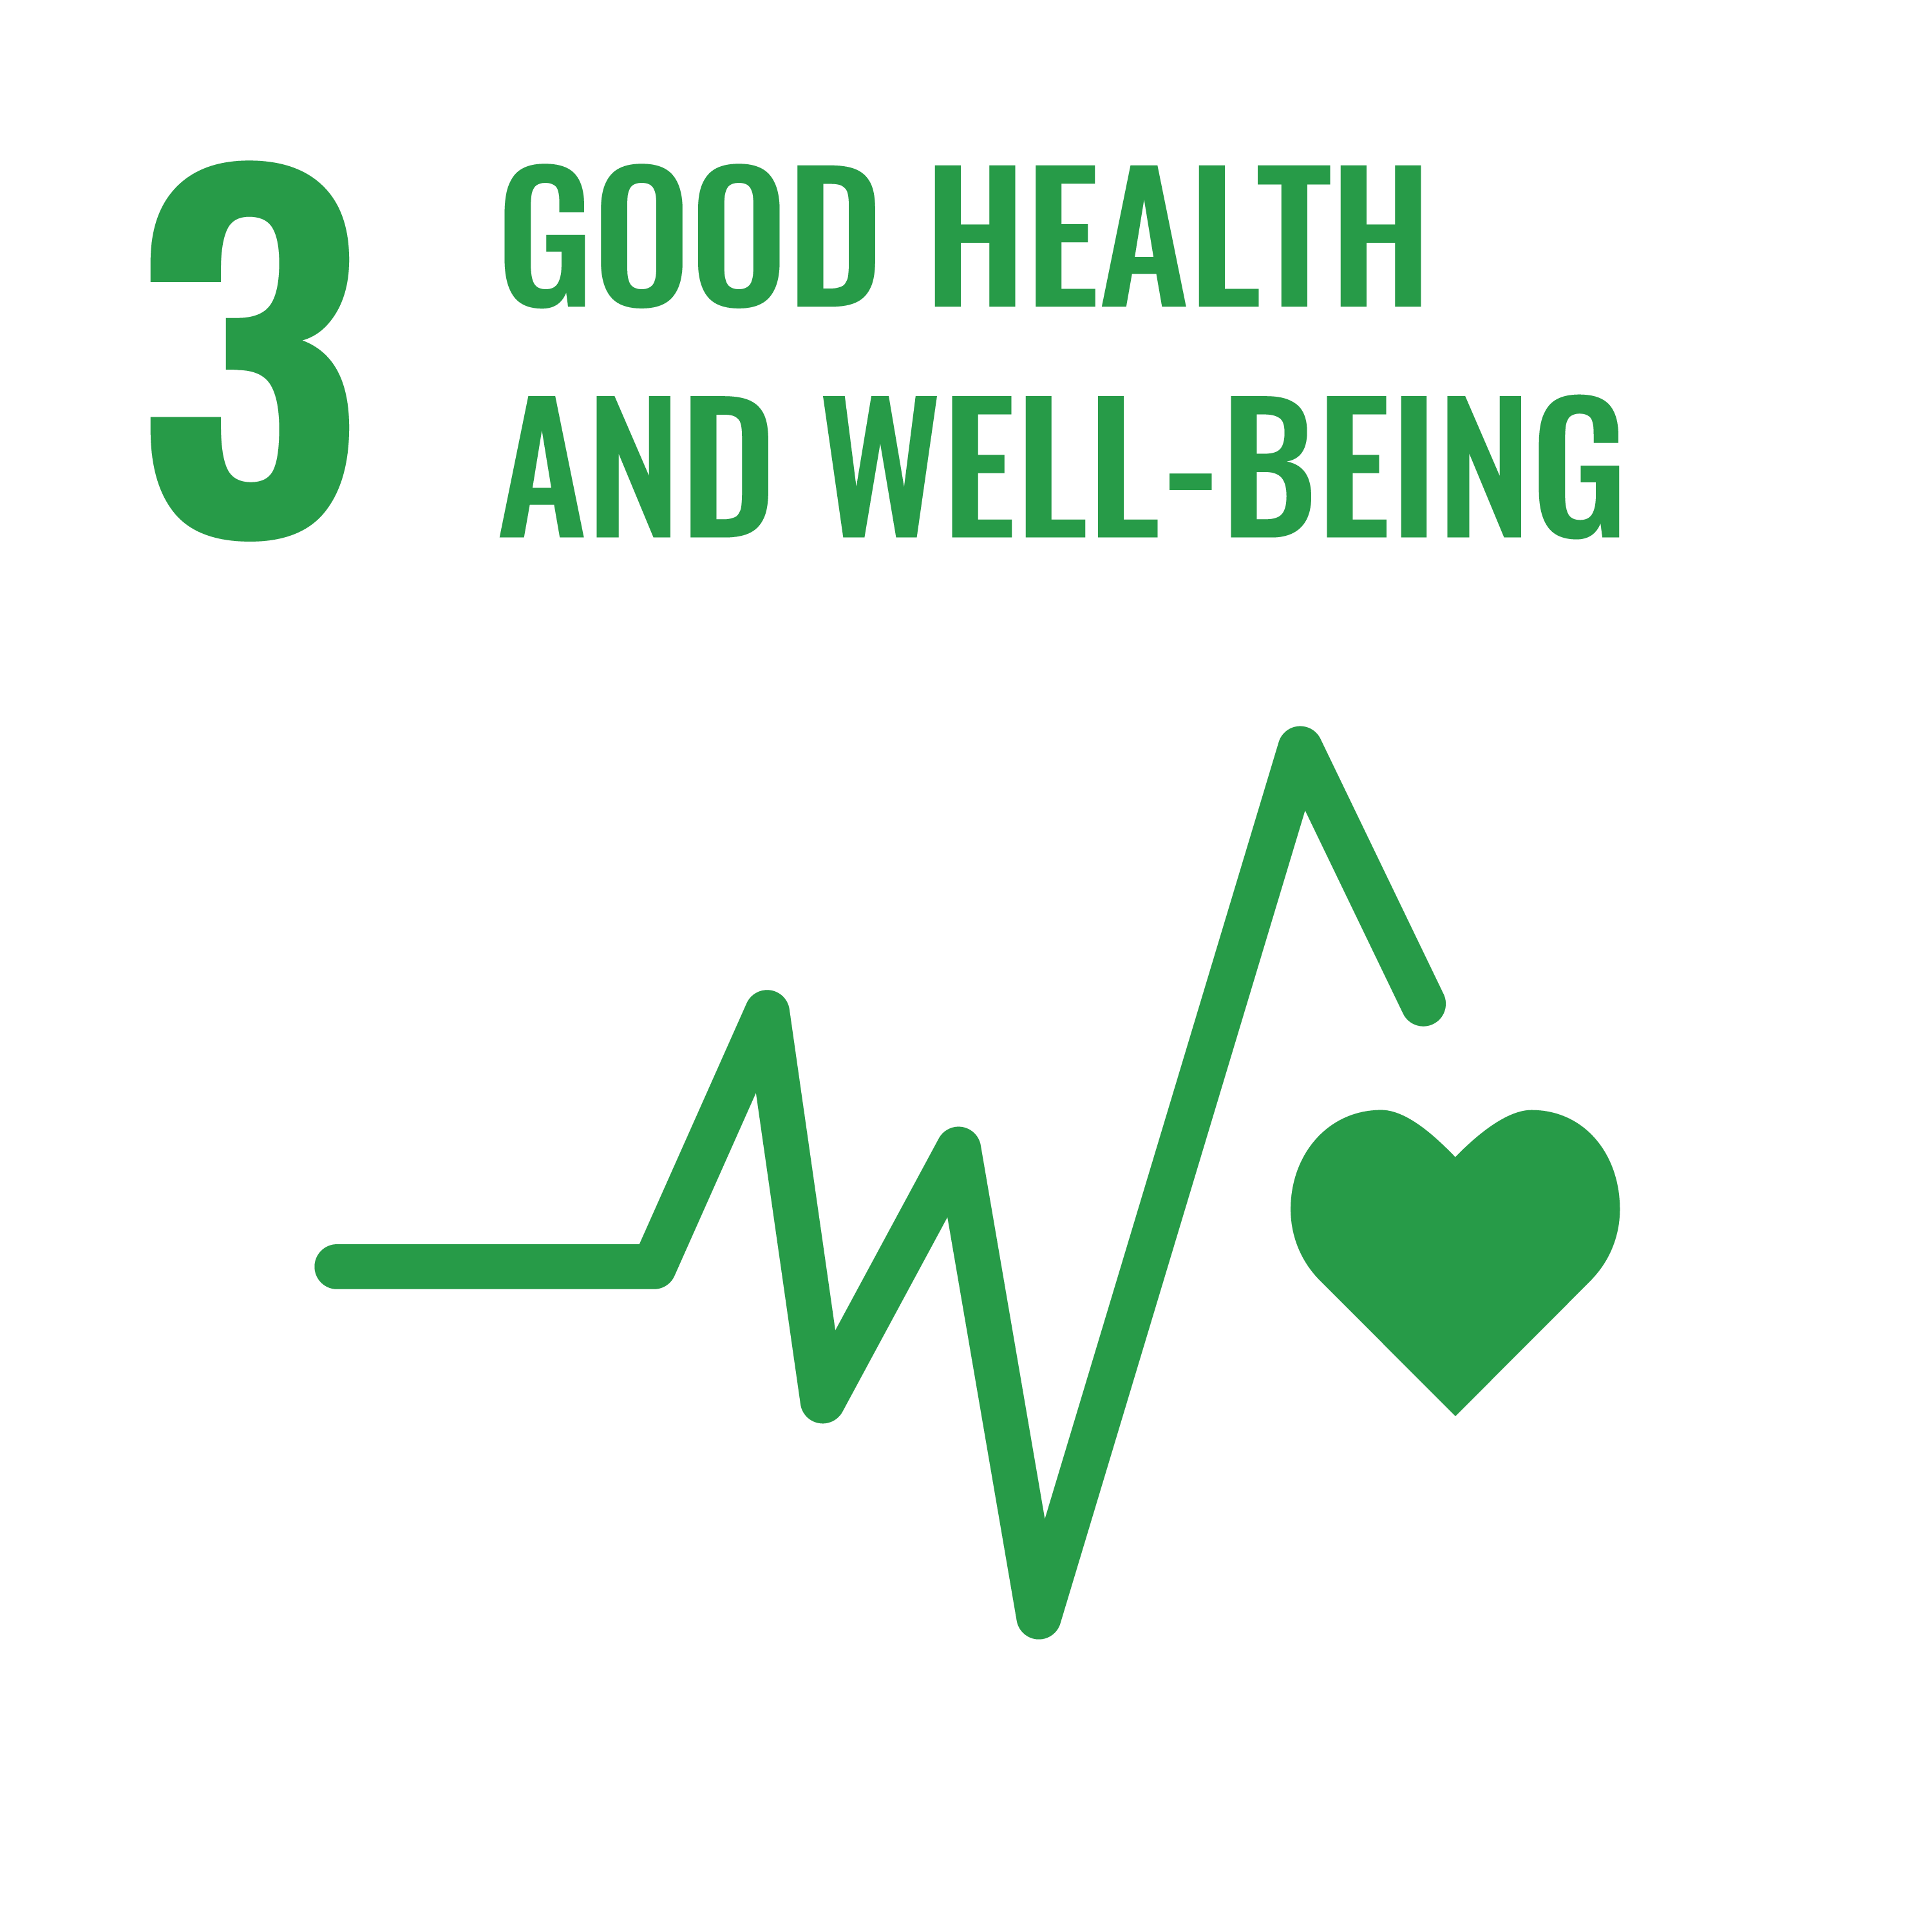
\includegraphics[width=\SDGsize]{Common/SDG_3_GoodHealth.png}~
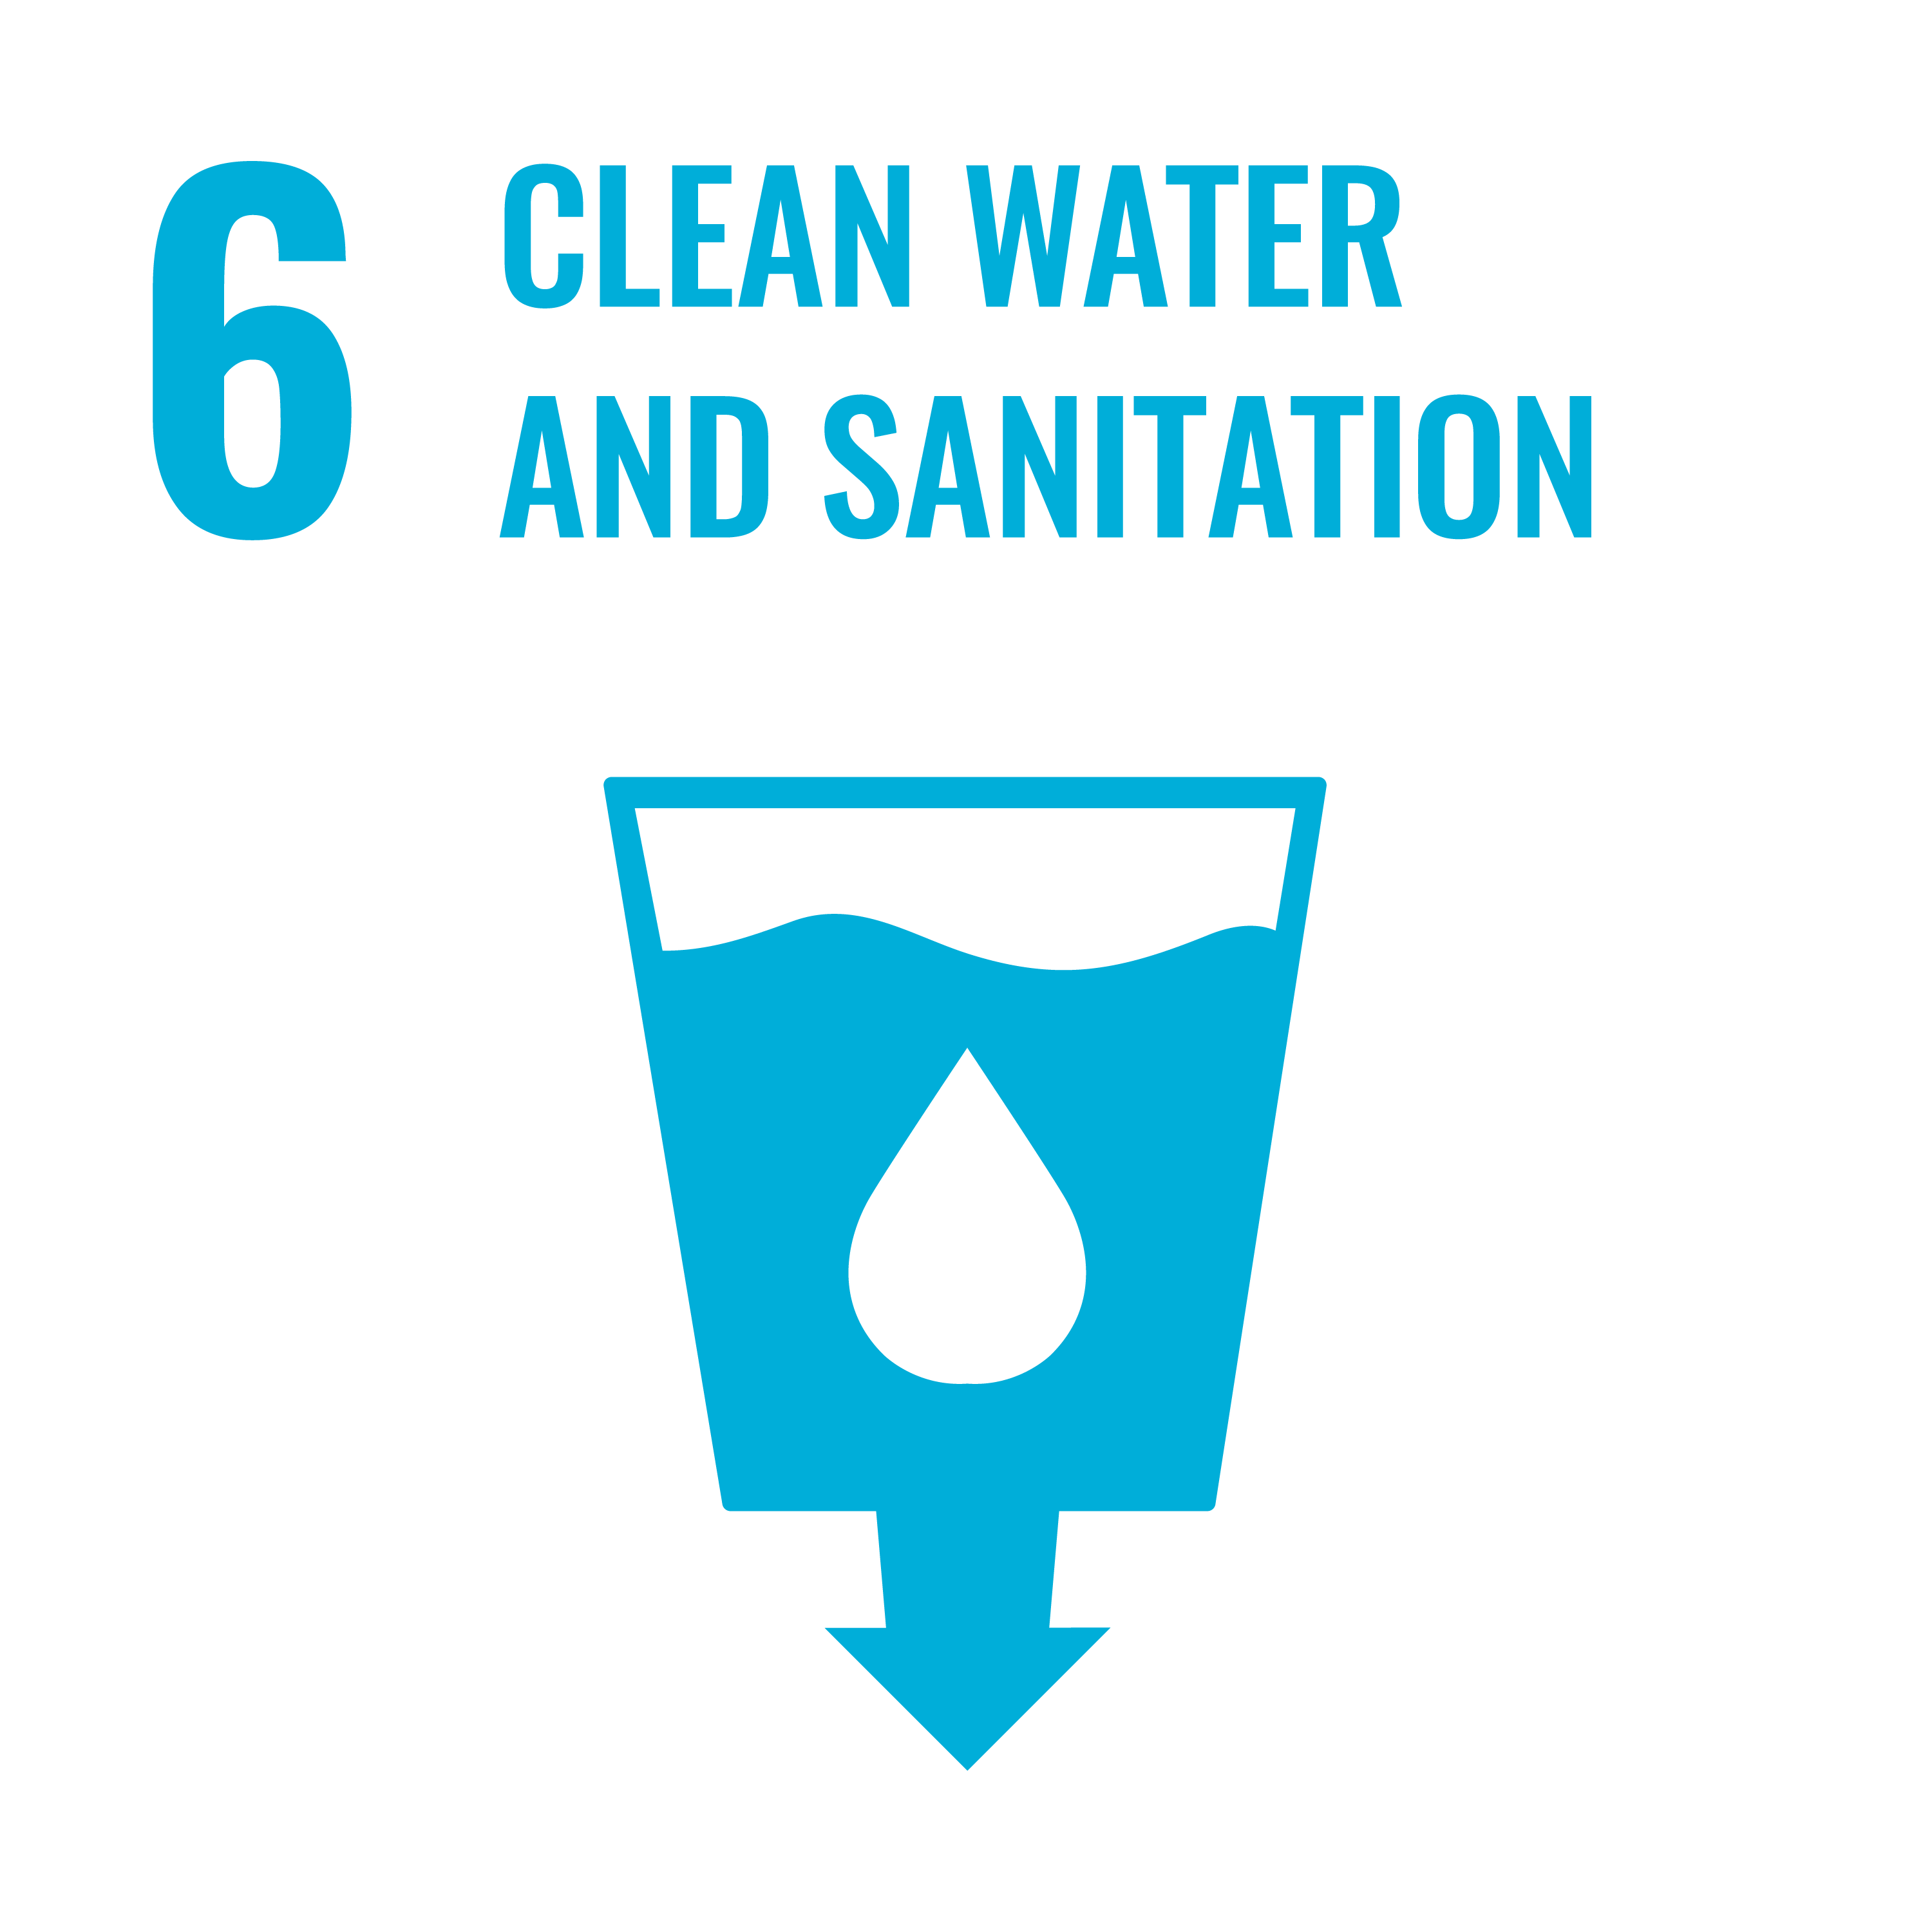
\includegraphics[width=\SDGsize]{Common/SDG_6_CleanWater.png}~
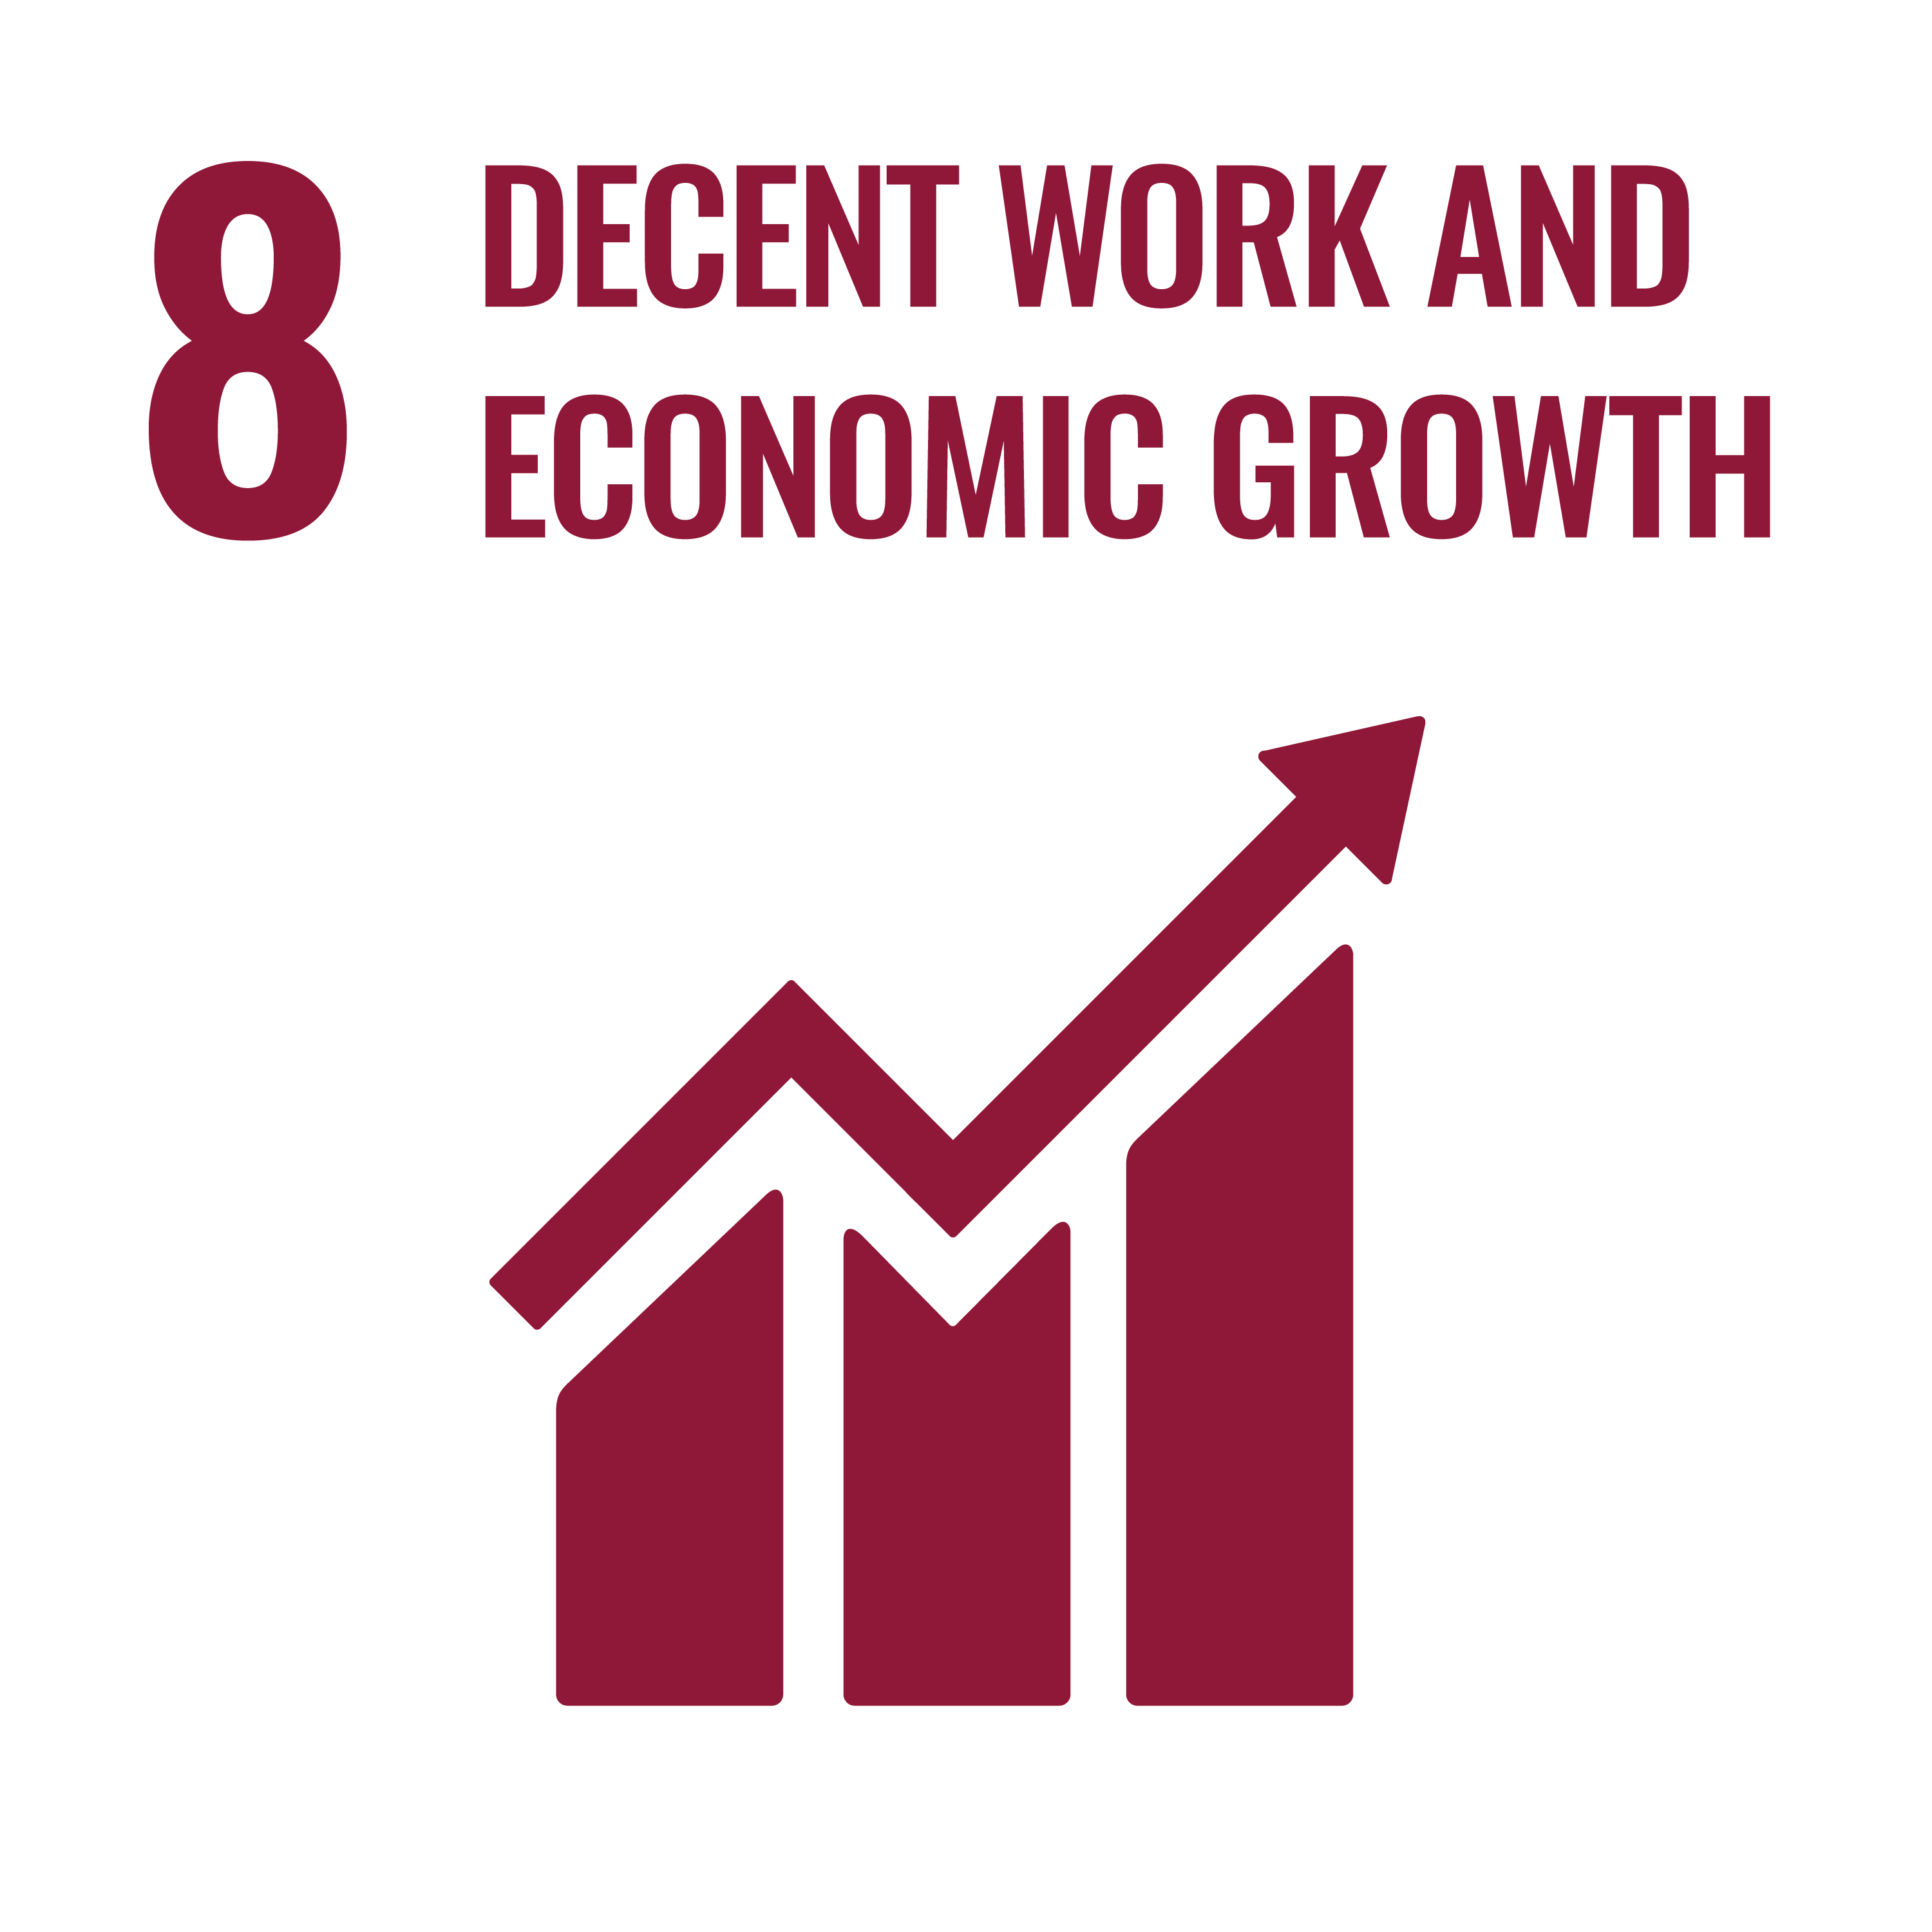
\includegraphics[width=\SDGsize]{Common/SDG_8_EconomicGrowth.png}~
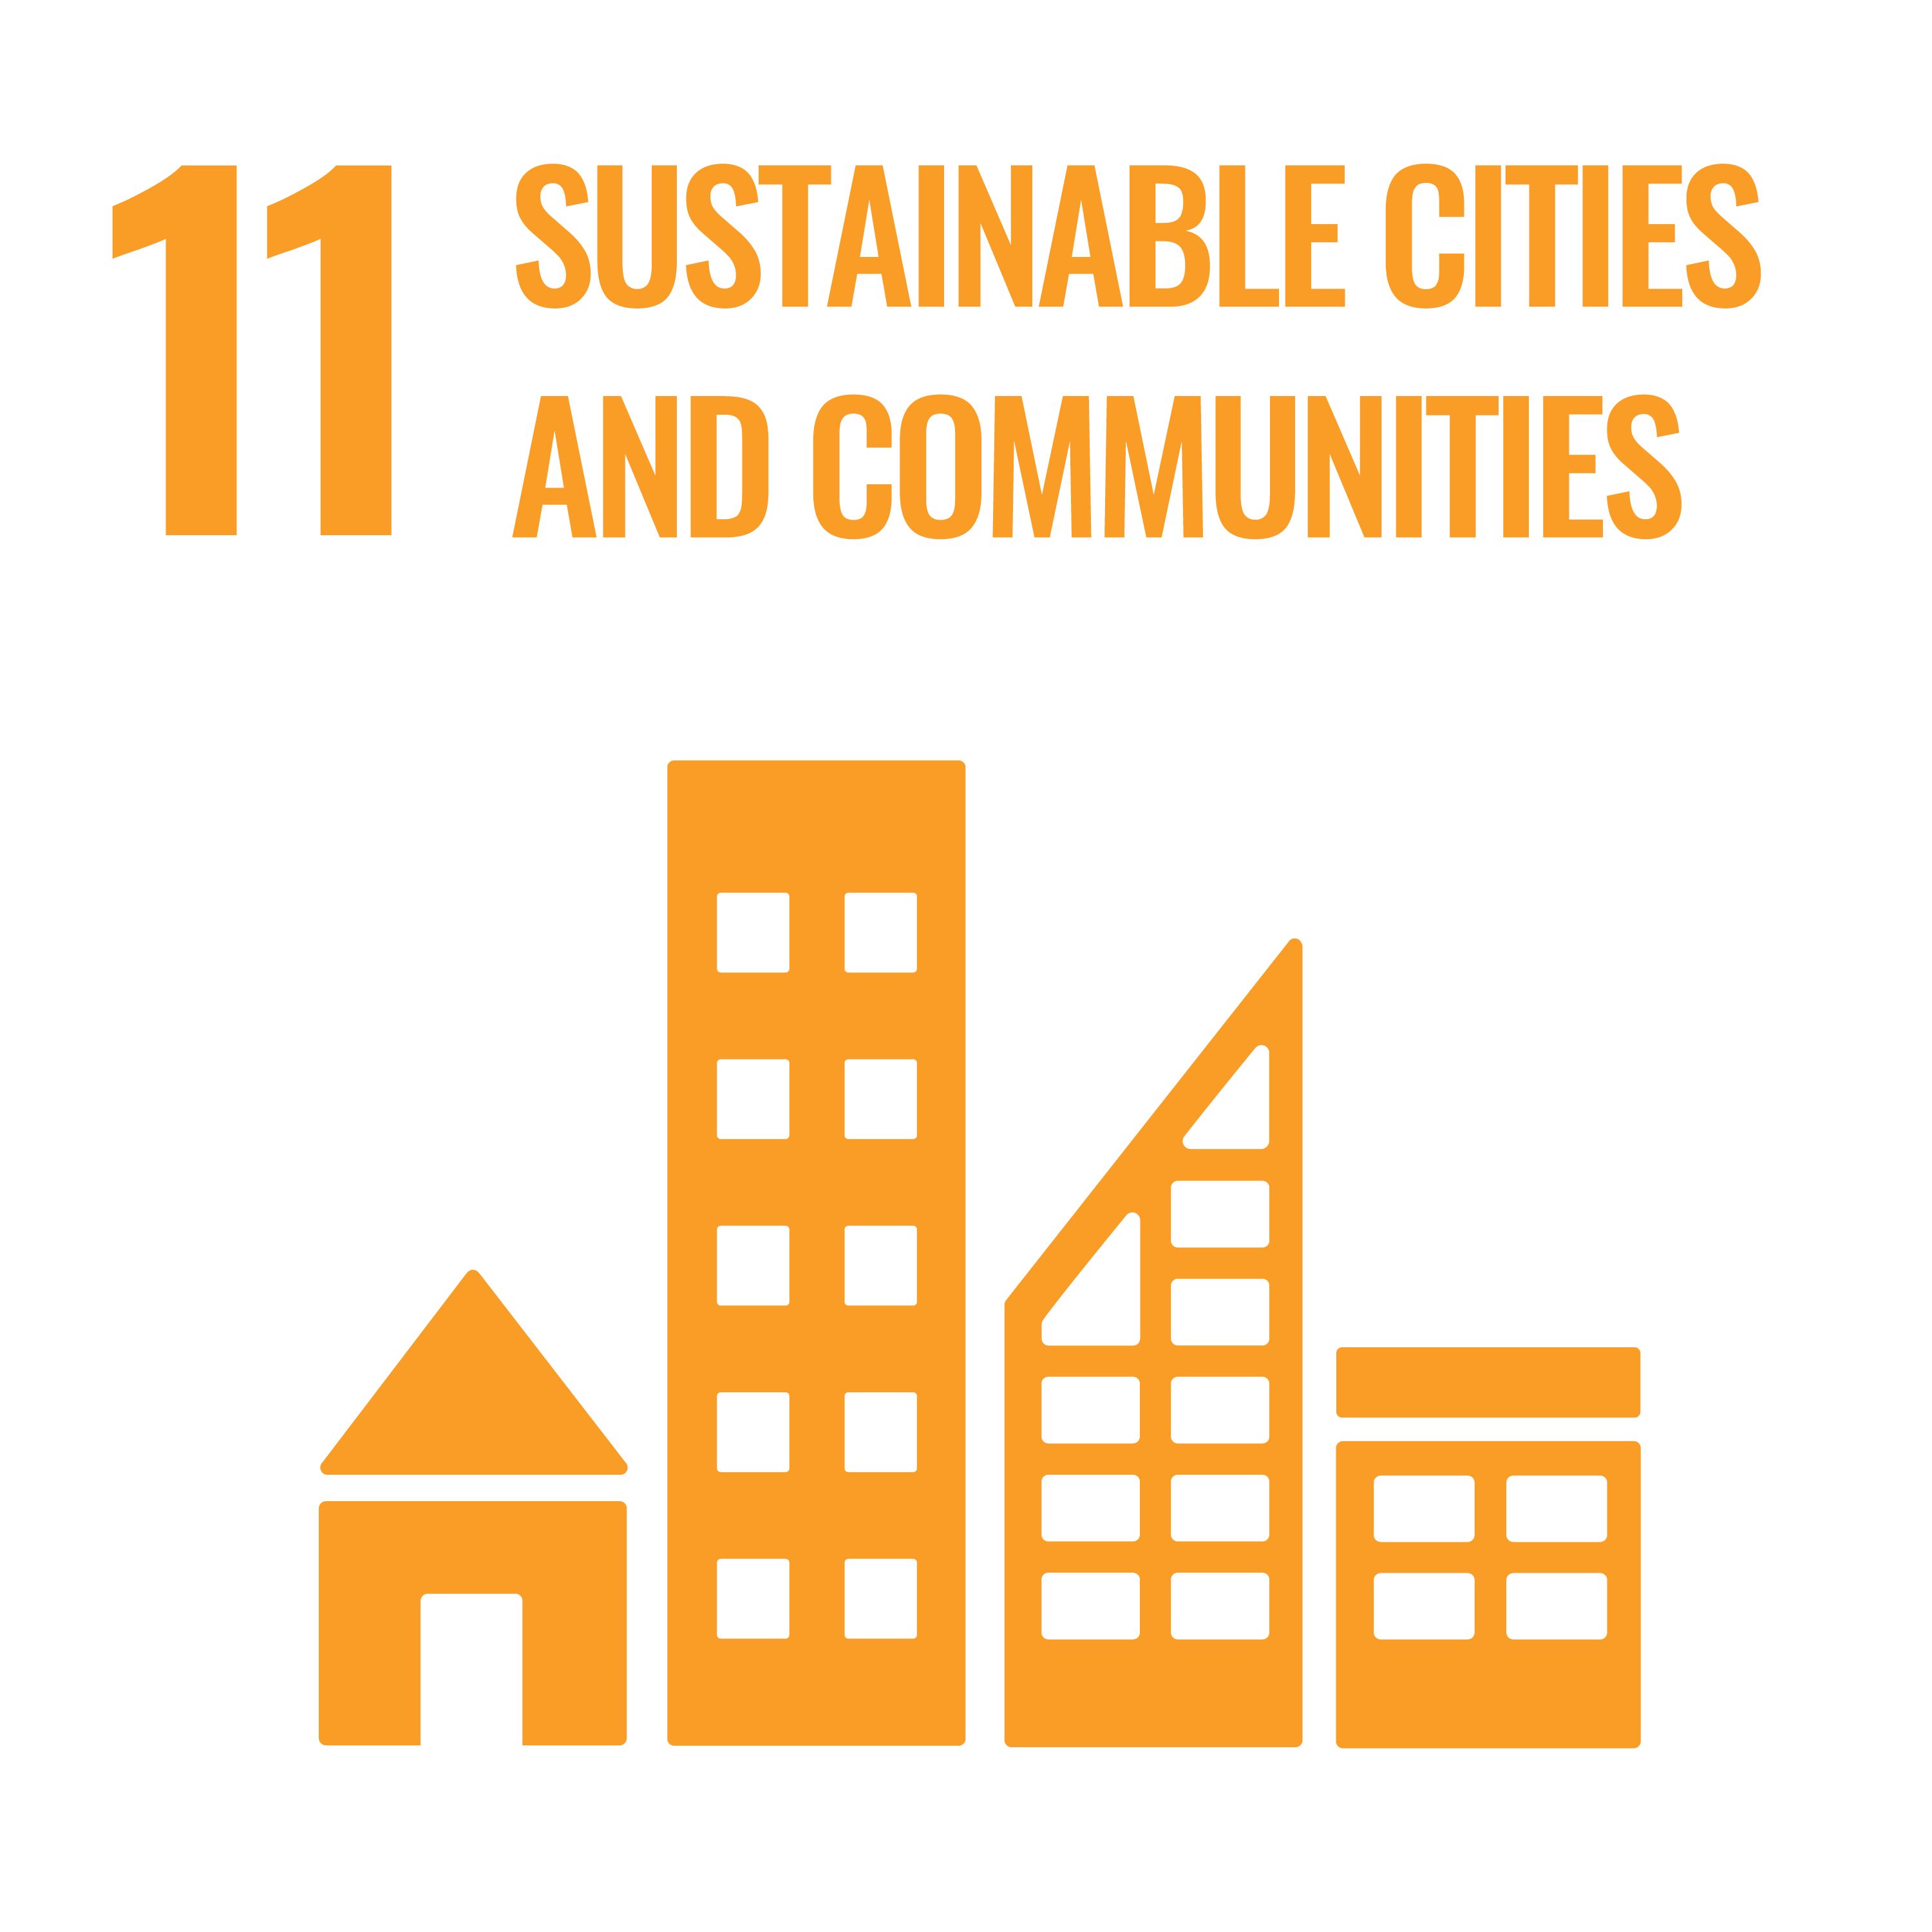
\includegraphics[width=\SDGsize]{Common/SDG_11_SustainableCities.png}~
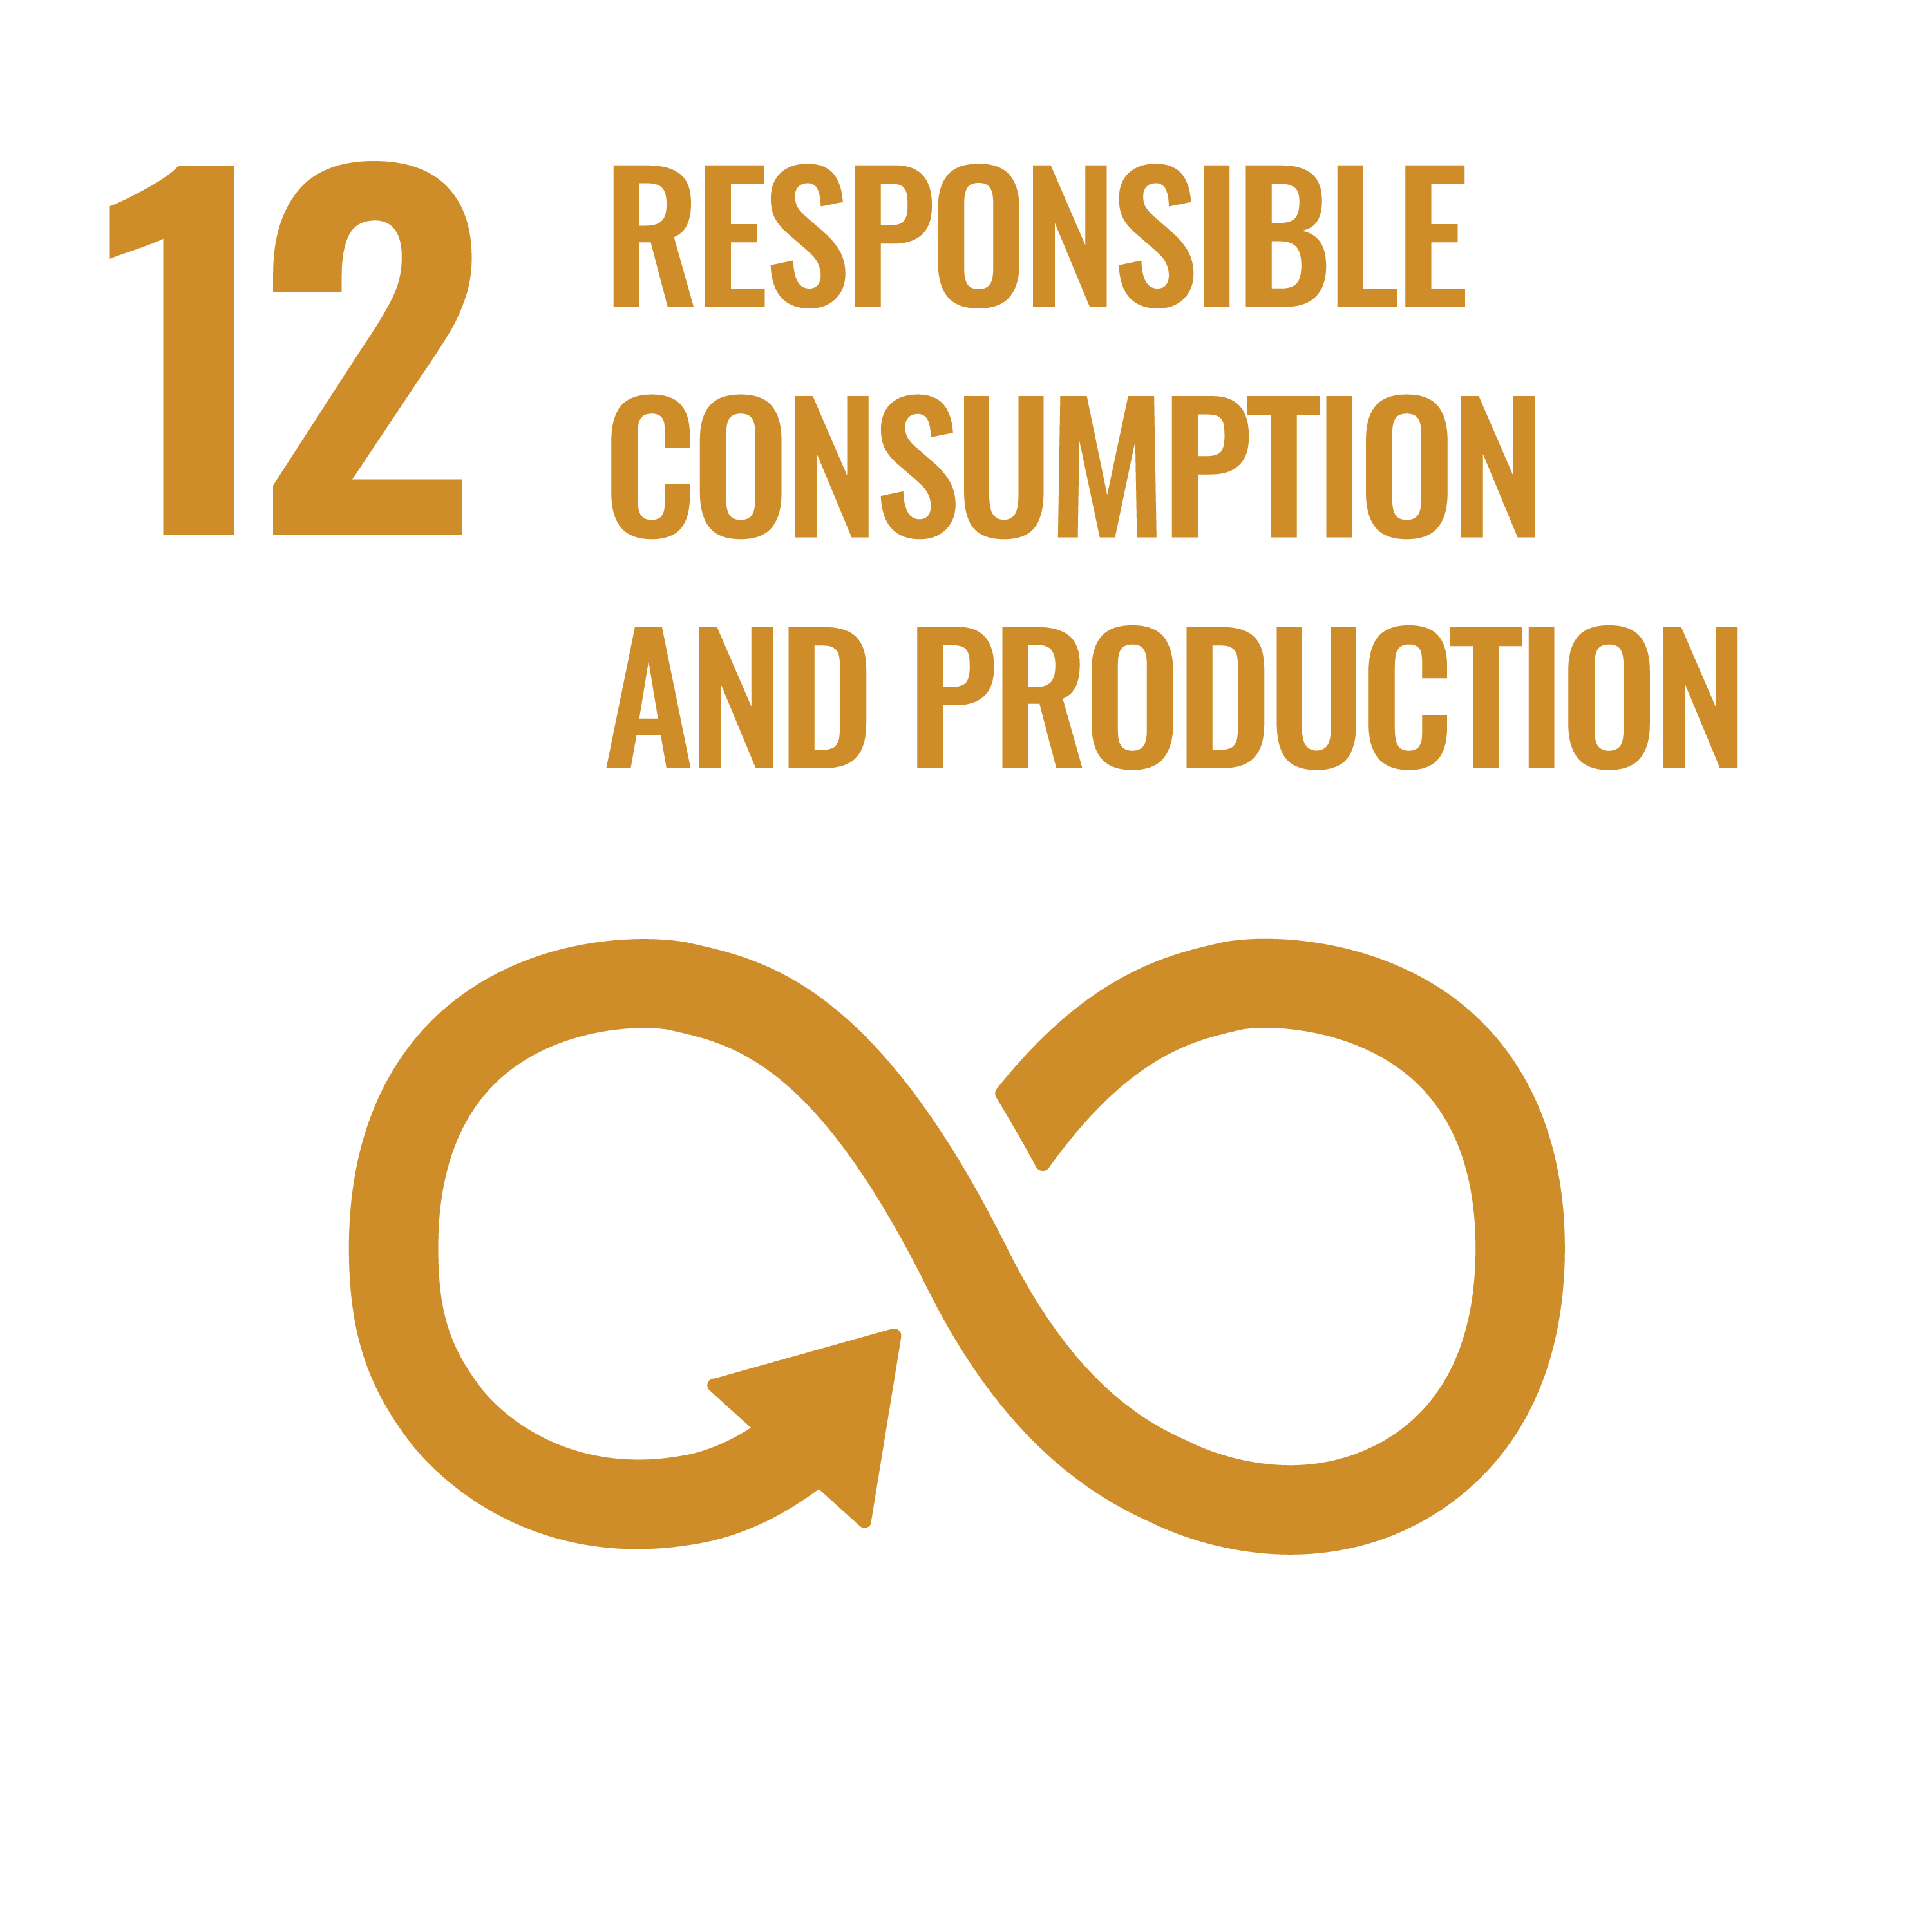
\includegraphics[width=\SDGsize]{Common/SDG_12_ResponsibleConsumption.png}~
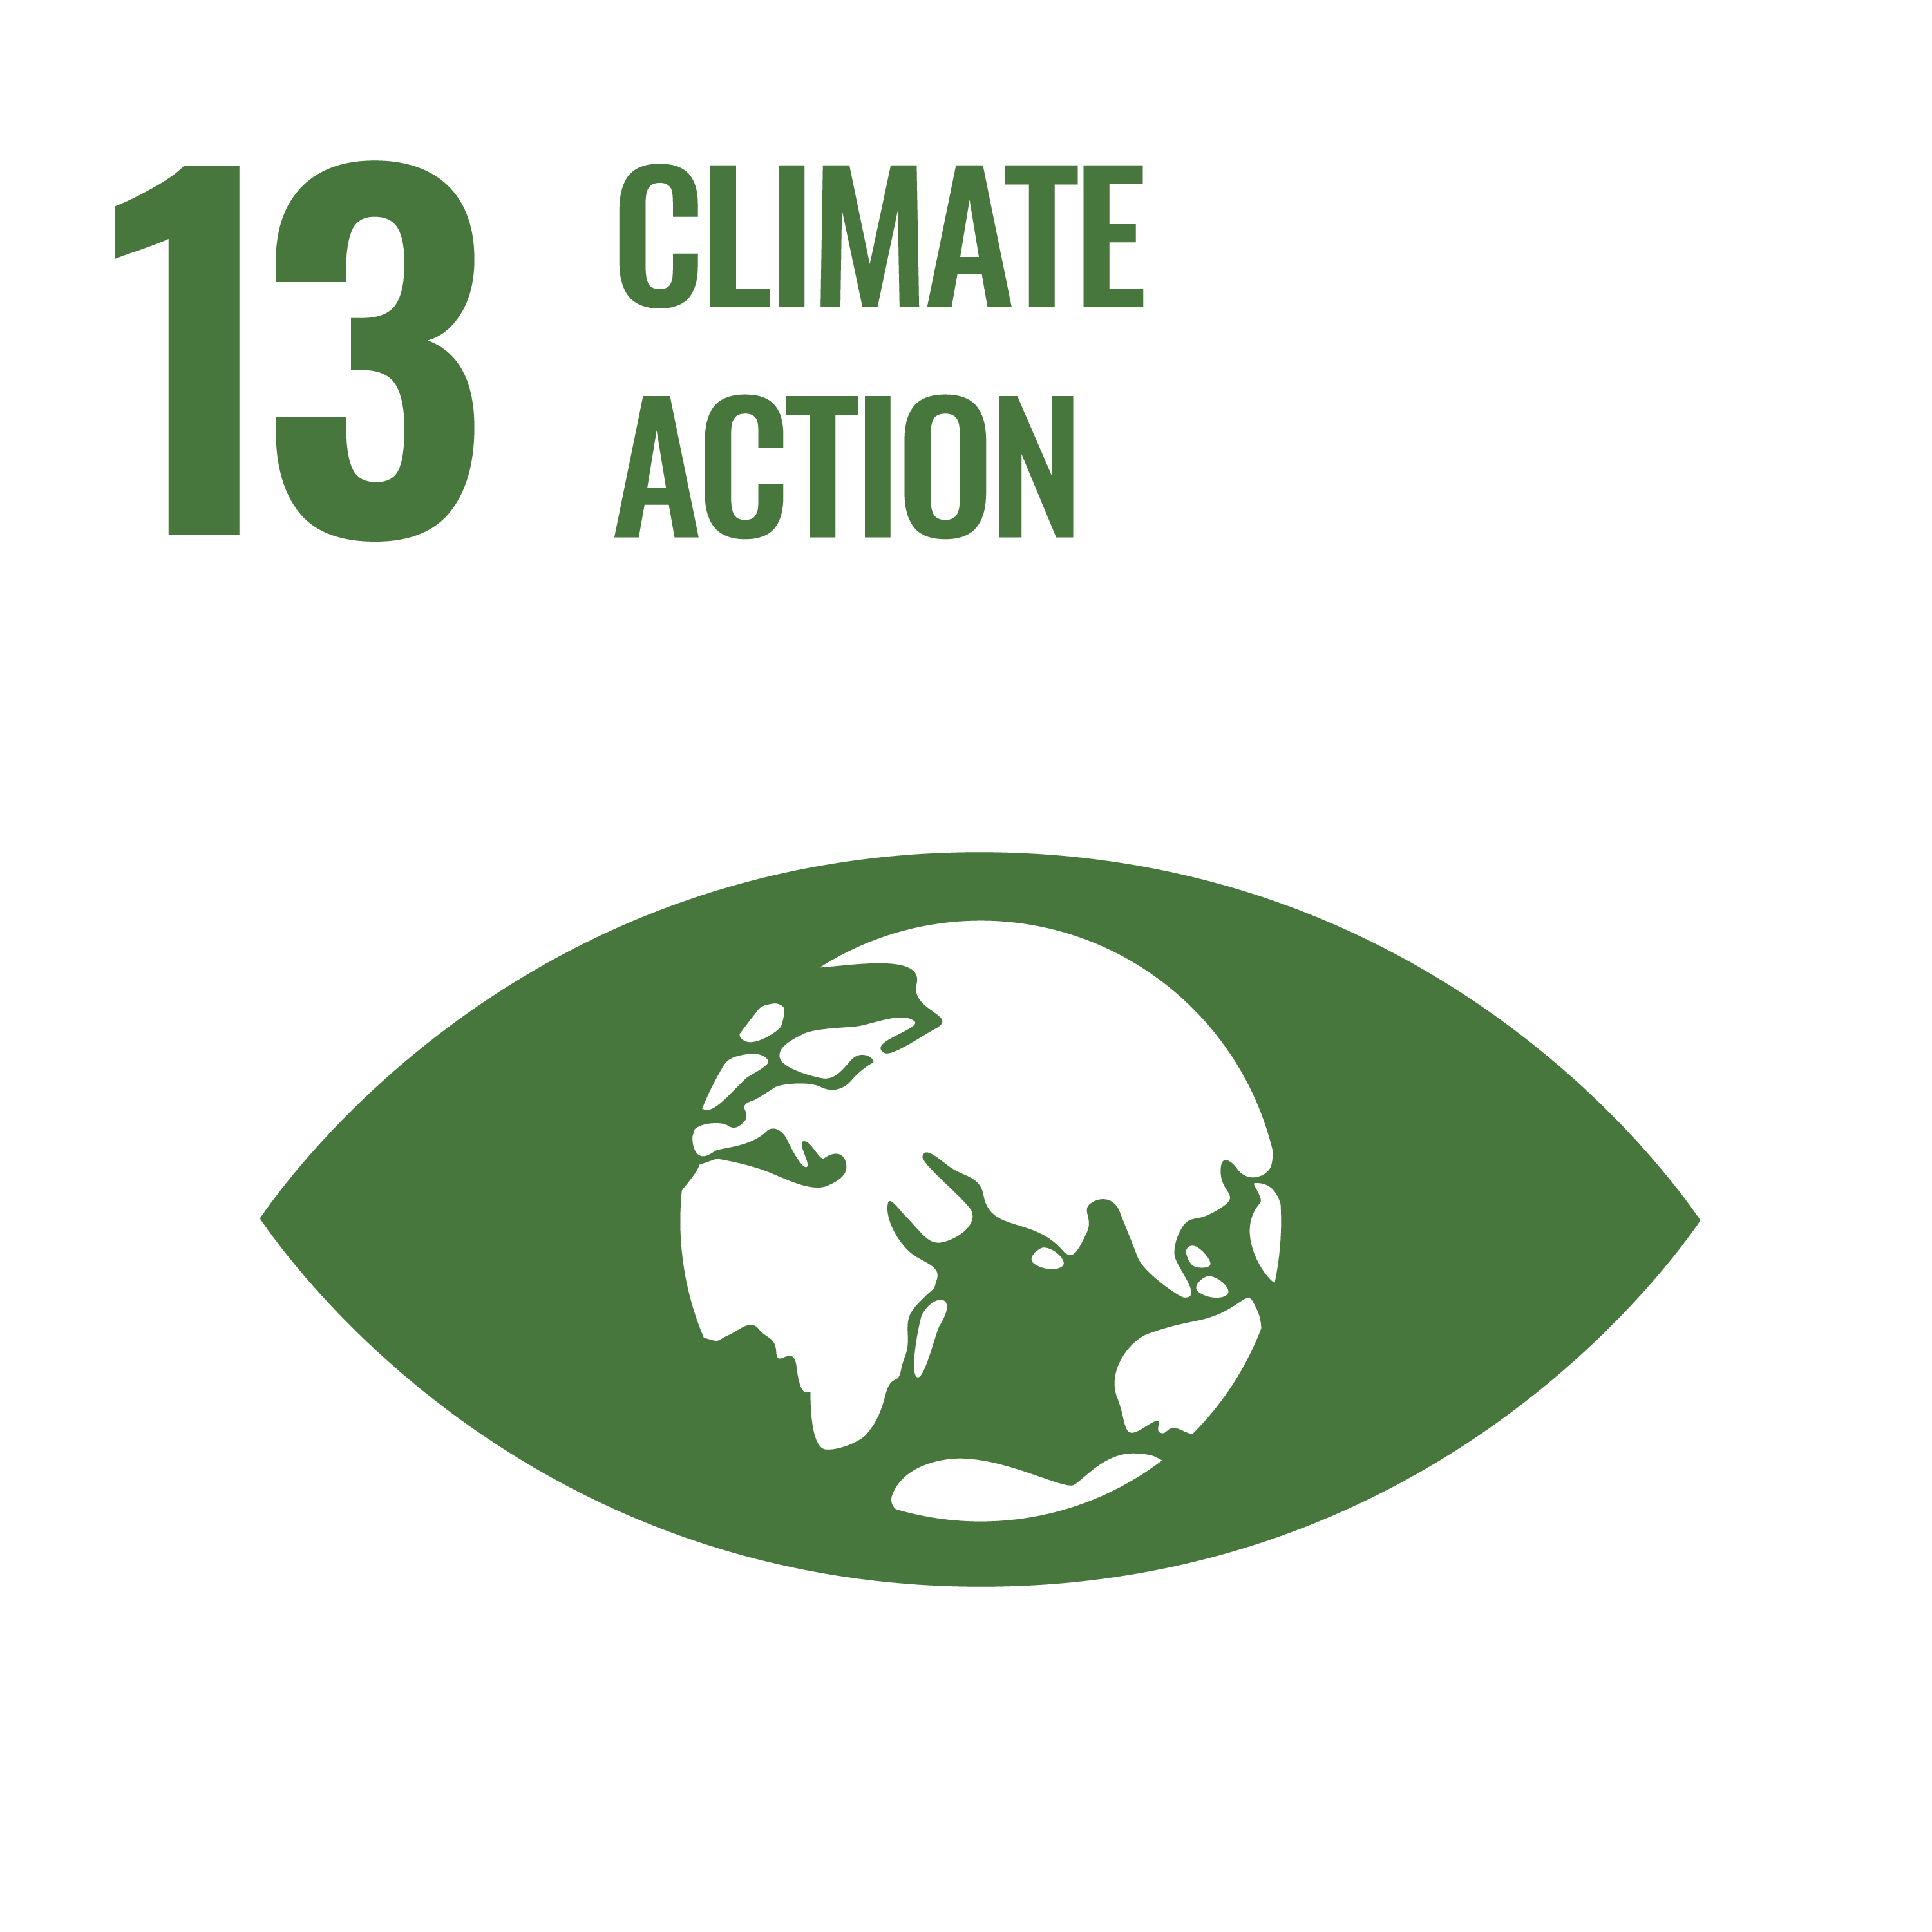
\includegraphics[width=\SDGsize]{Common/SDG_13_ClimateAction.png}~
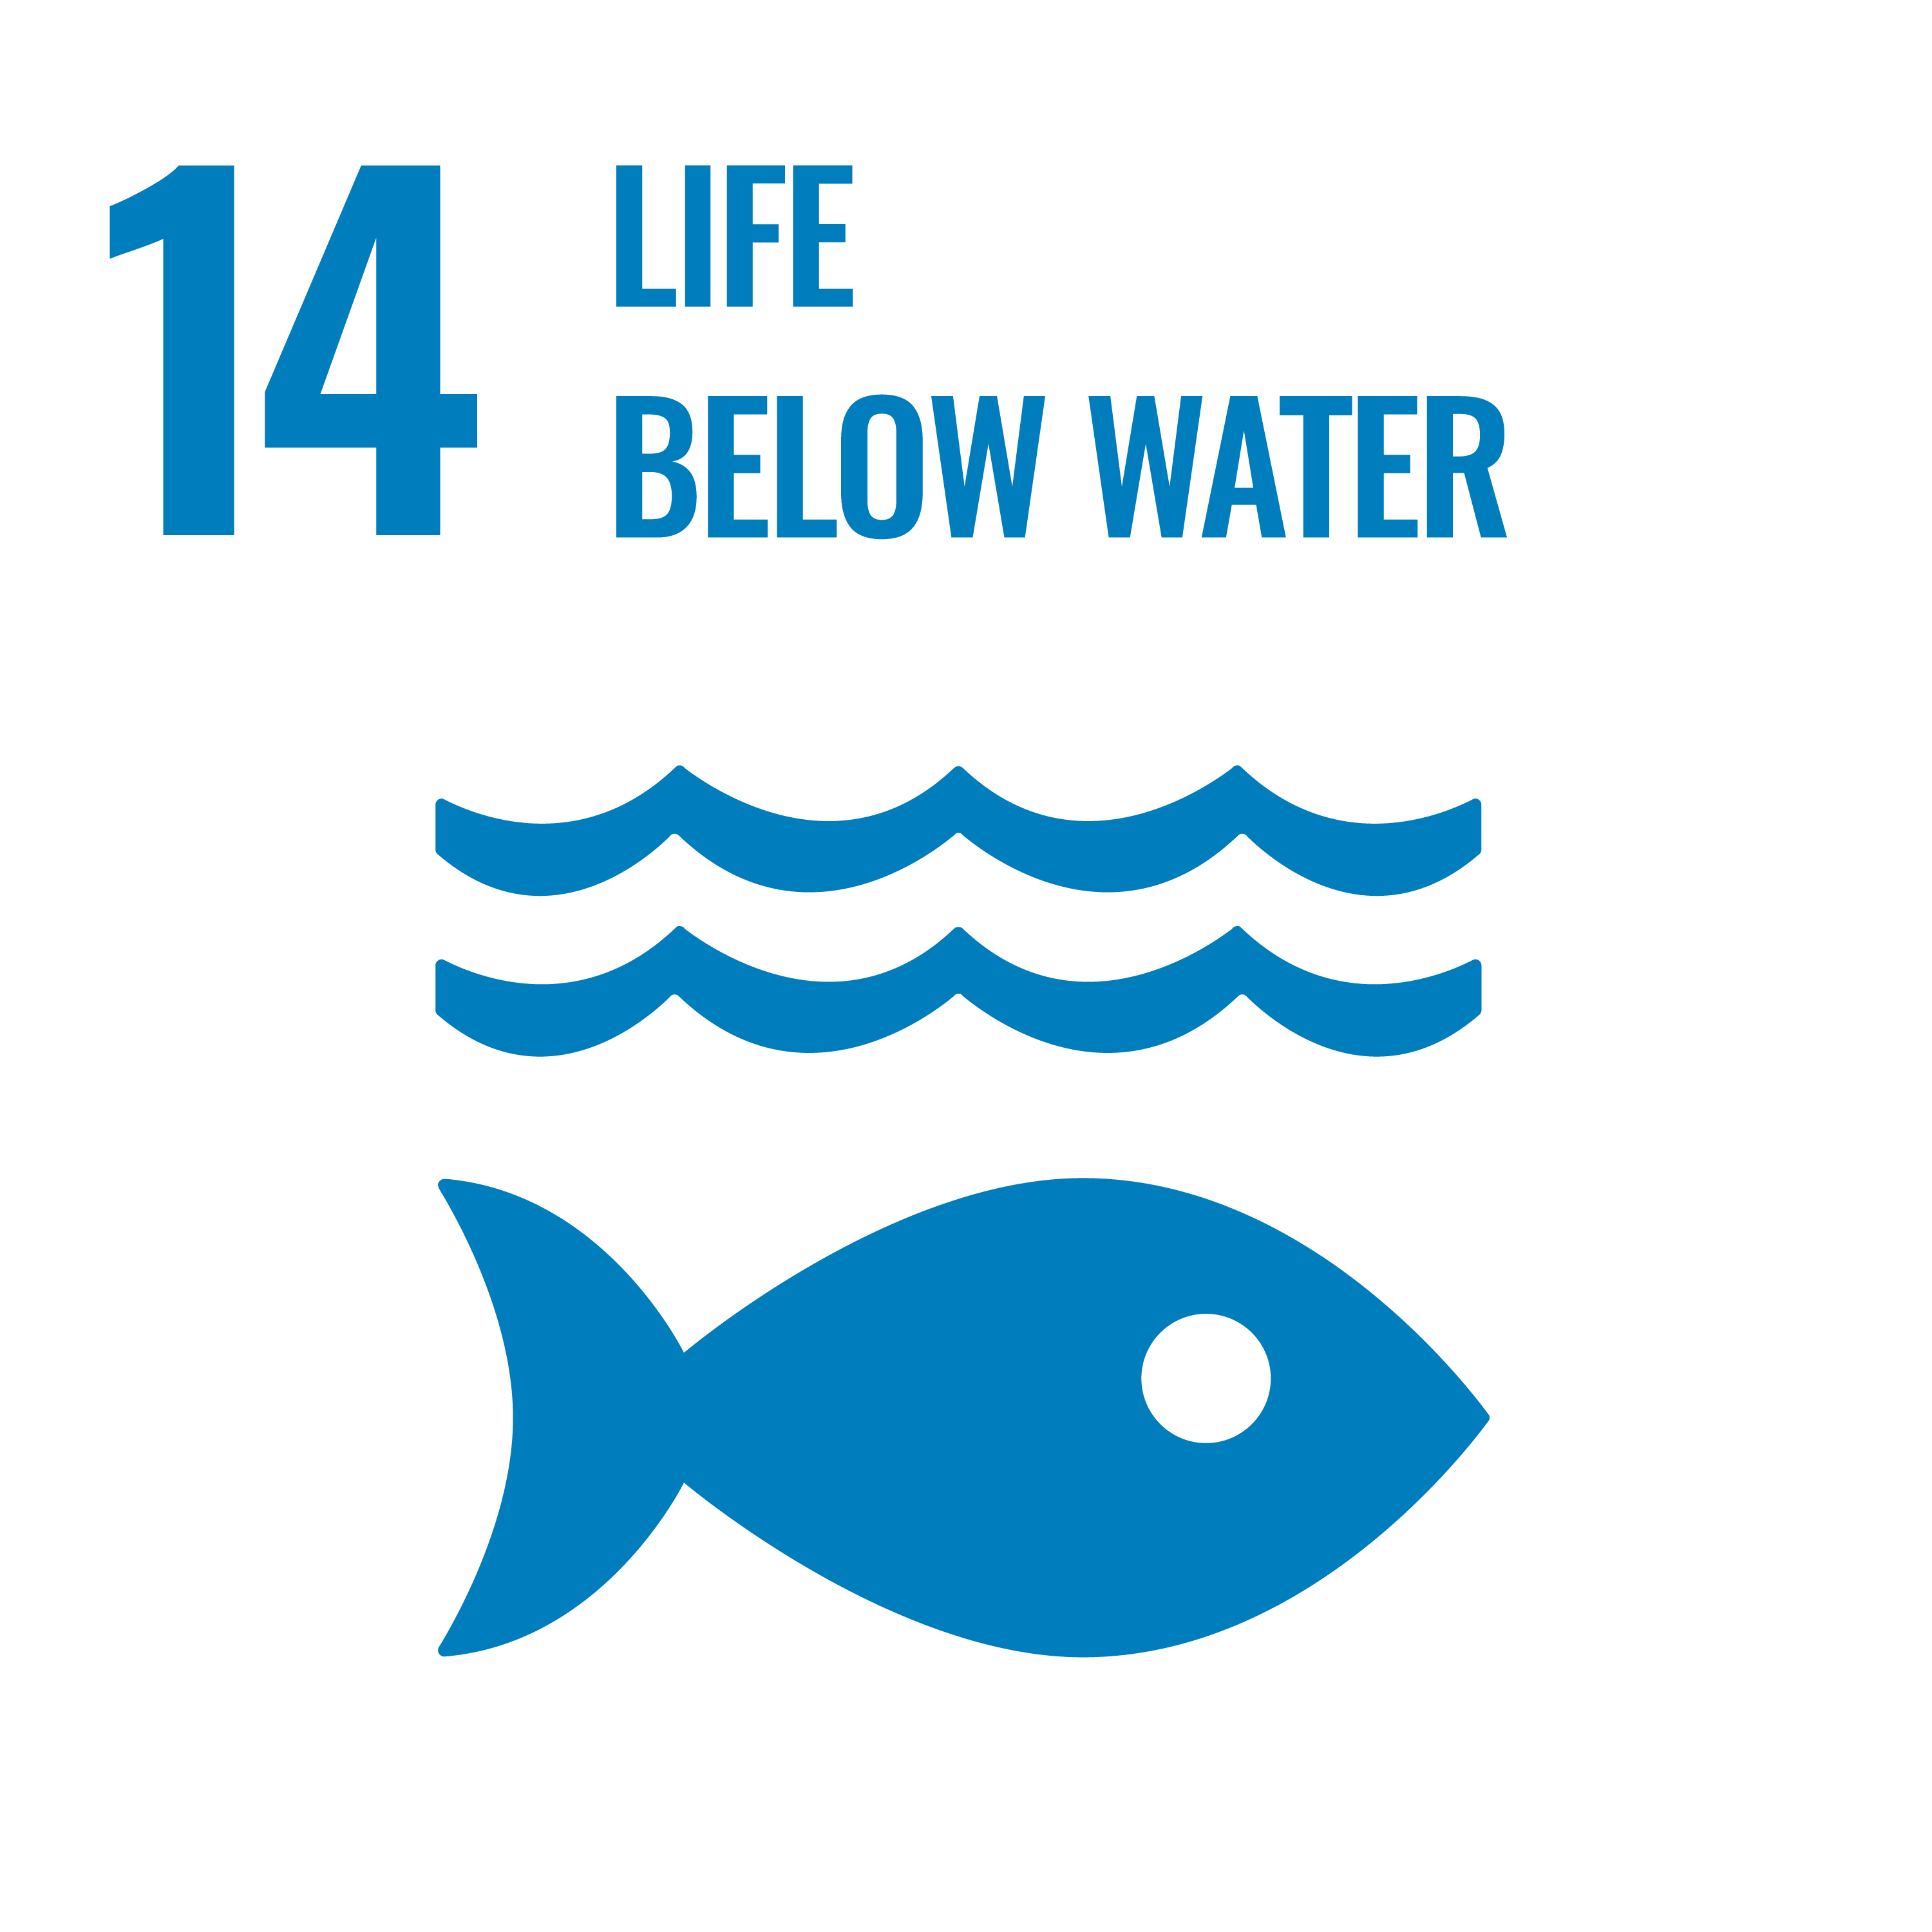
\includegraphics[width=\SDGsize]{Common/SDG_14_LifeBelowWater.png}~
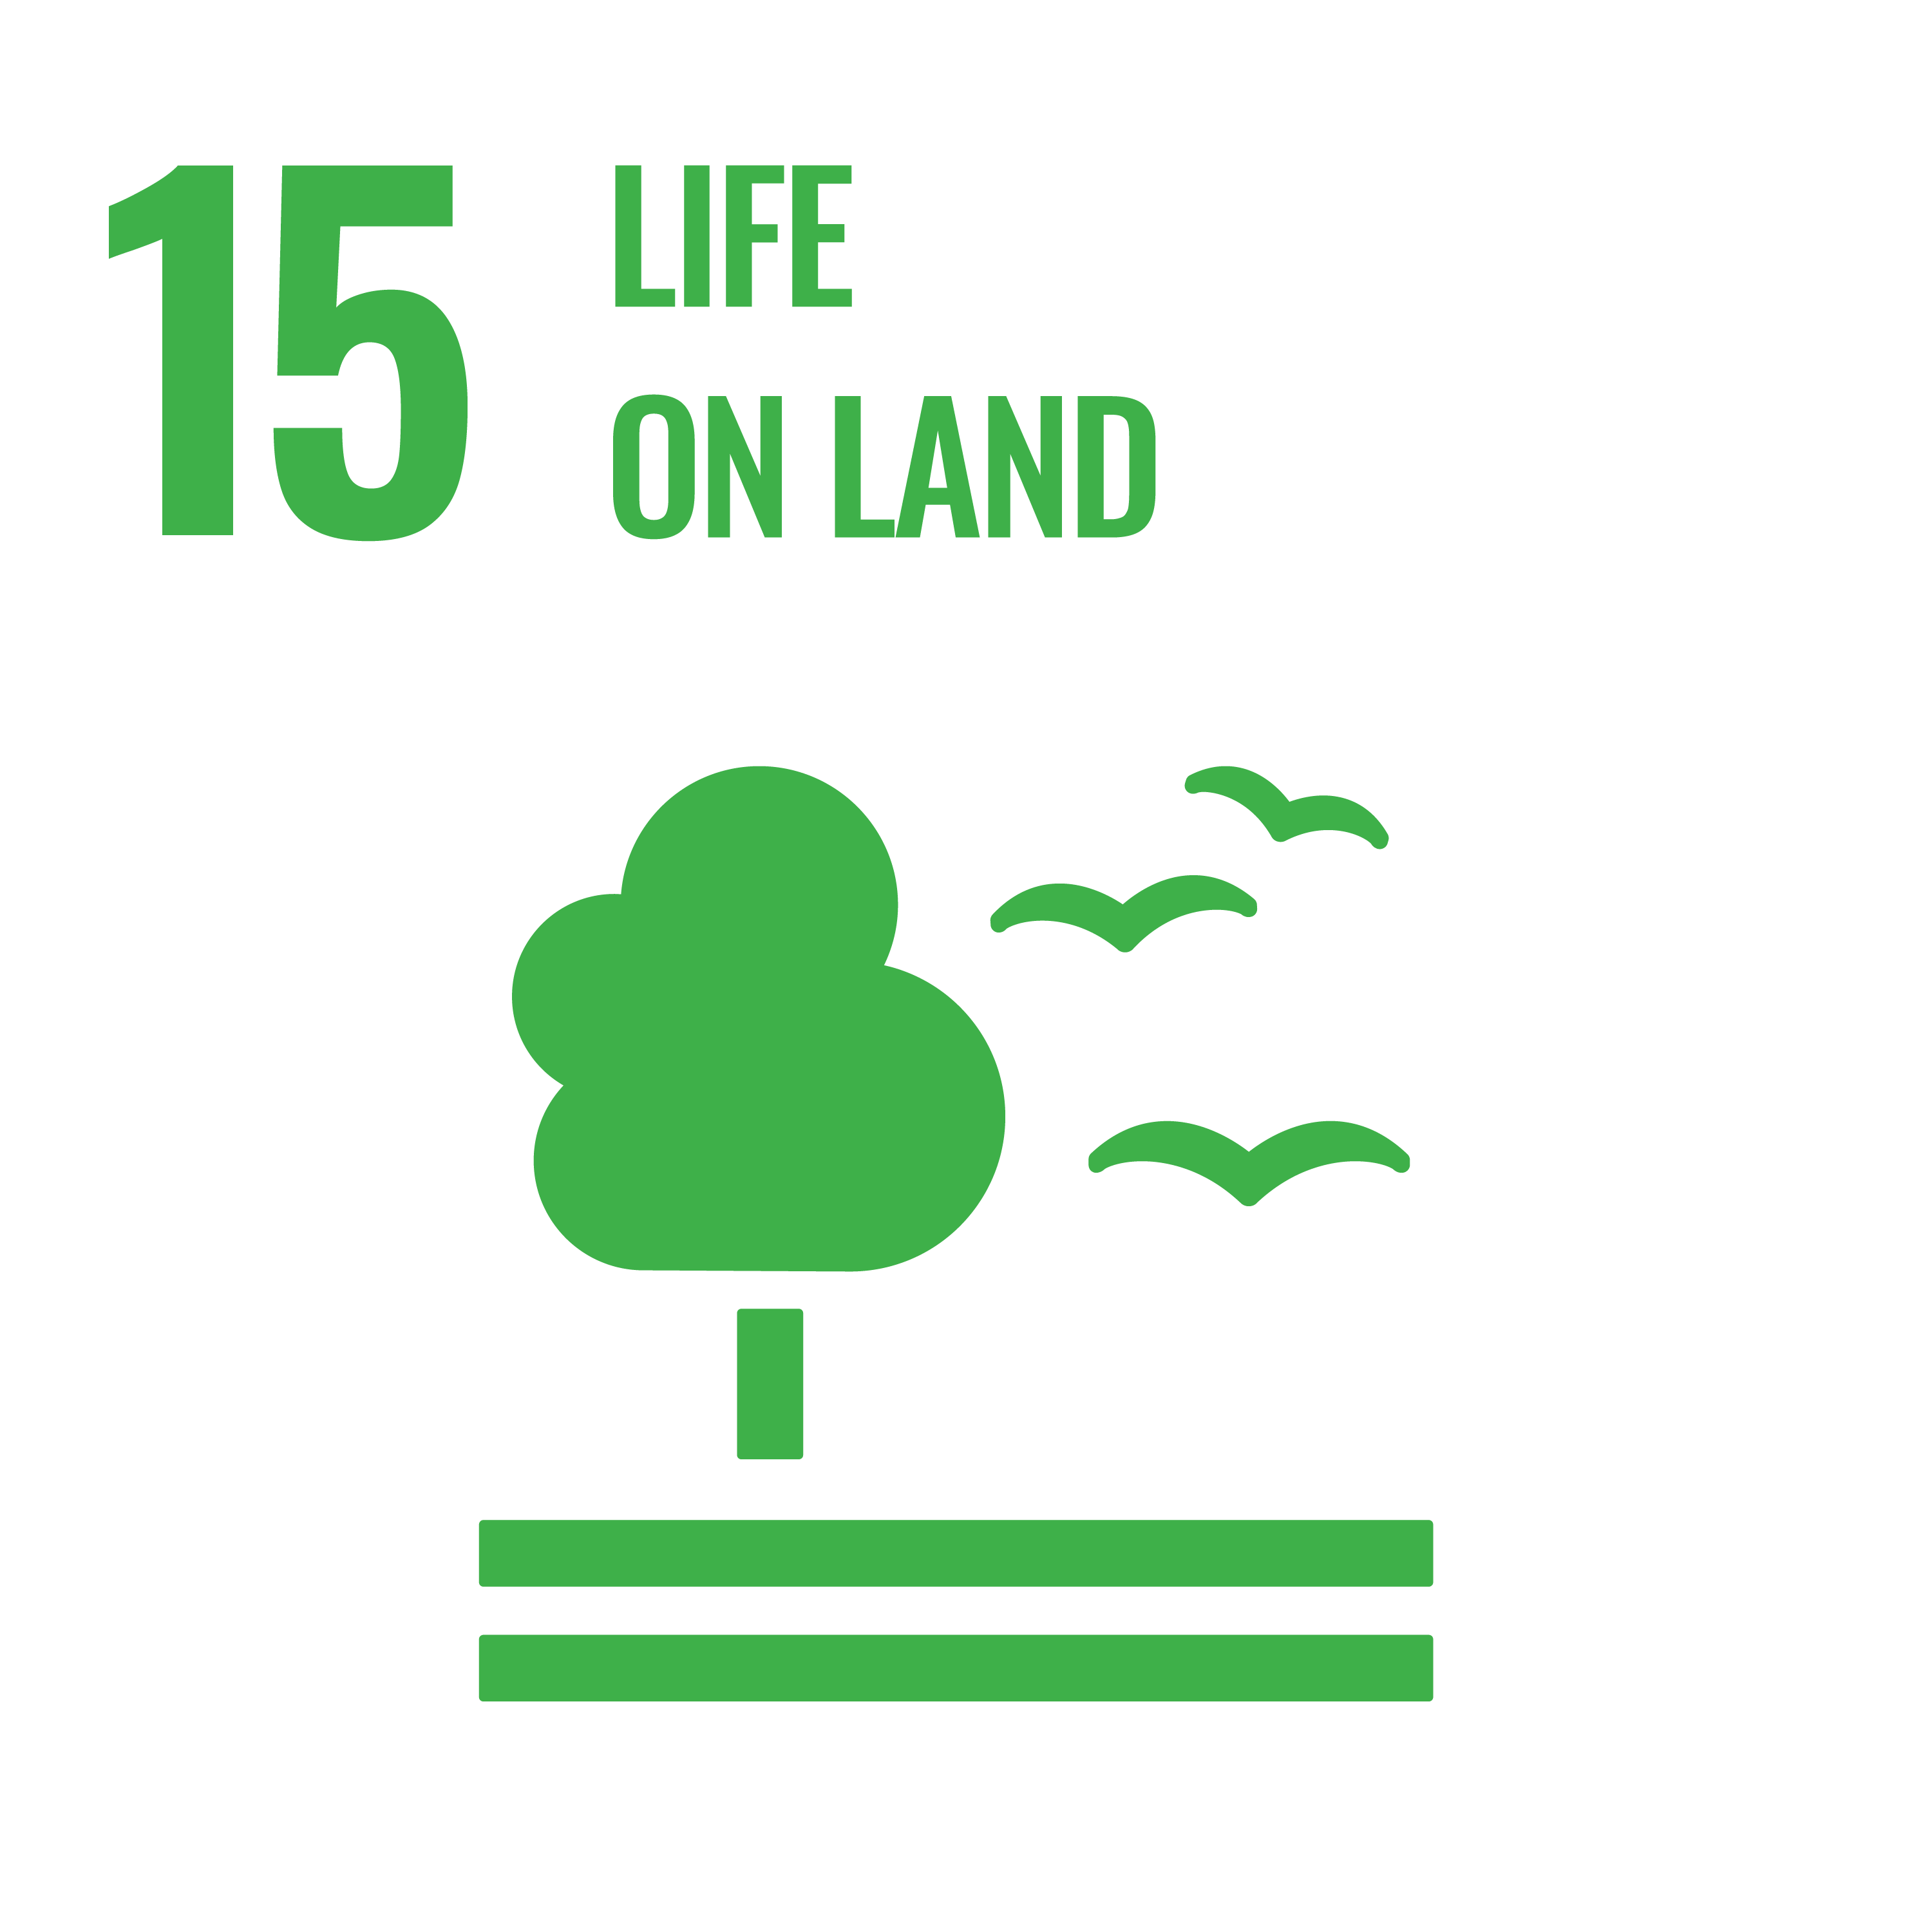
\includegraphics[width=\SDGsize]{Common/SDG_15_LifeOnLand.png}
\end{center}

%%%%%%%%%%%%%%%%%%%%%%%%%%%%%%%%%%%%%%%%

\exSum
 \noindent

Half of the world's GHG emissions, and over 90\% of global water stress and biodiversity loss events, are due to the extraction and processing of raw materials~\cite{EURaw}. Although most extracted materials are slated for the energy or agriculture sectors, the tiny remainder directly associated with consumption of goods and services is nevertheless responsible for 18\% of emissions due to EU consumption~\cite{EURaw}. Mitigating the climate impacts of the extraction, processing and trade of raw materials is a priority for the resilience of the EU~\cite{EURaw}, and should be one also for the World climate agenda.

The generation of waste is a direct consequence of material consumption and is aggravated by constraints in the various stages of production, distribution, usage and repair, disposal or recycling of consumables. Waste has severe impacts on life on the land and sea, often destabilizing local ecosystems, and contributes to climate change, thus destabilizing the global ecosystem. Accumulations and inefficient disposal of waste products also directly affect the health of individuals and communities, when ground water and air are polluted with toxic agents, leading to a large cost in terms of lives lost and disease burden on society. 

In an attempt to curb the footprints left by the generation of waste, the concept of a circular economy has been proposed~\cite{CircularEconomy}.  Any such proposal must also be established in parallel with a will to reduce waste at source through sustainable procurement, repair and reuse, and must serve as a transition to this final solution.  Circular economy can significantly aid in this transition to reducing waste, as it is quick and easy to implement, it has a strong educational role, and is economically favourable.  However even a fully circular economy has some dissipation, and signatures of this energy waste need to be addressed separately and reduced~\cite{Forbes,SocialEurope,WRI}.

Maximizing the sustainability of the use cycle of resources should be a priority of the \ACR\ community.

{\footnotesize\bf Thanks to Enrico Cennini and Quentin Salvi for original material and references.}\\
%%%%%%%%%%%%%%%%%%%%%%%%%%%%%%%%%%%%%%%%

\clearpage
\begin{reco2}{\currentname}
{
\begin{itemize}[leftmargin=3.5 mm]
\item Limit purchases; service appliances regularly; share, repair, reuse and refurbish to minimize waste; sort and recycle.

\item Read the sections on computing (\sref{sec:Computing}), energy (\sref{sec:Energy}), food (\sref{sec:Food}), and research infrastructure and technology (\sref{sec:Technology}).
\end{itemize}
}
{
\begin{itemize}[leftmargin=3.5 mm]
\item Adopt life-cycle assessments and associated tools to assess environmental impact of all activities.

\item Institute sustainable purchasing, usage and end-of-life policies in the management of group consumables,  office supplies and single-use plastics \eg in conference events (see also Section~\ref{sec:CateringTableware} and Best Practice \ref{bp:PlasticFreeConf}).
\end{itemize}
}
{
\begin{itemize}[leftmargin=3.5 mm]
%\item Adopt life-cycle assessment and associated tools to limit consumption and institute sustainable purchasing, usage and end-of-life policies for materials; consumables, such as office supplies, single-use items and cleaning products; and electrical and electronic equipment.

% \item Incentivise and support repair, reuse, reclaiming of materials, donation where viable, and recycling.
\item Prioritise suppliers instituting sustainable sourcing and operating policies, with a particular focus on the raw materials processing stage (see Best Practice~\ref{bp:SustainableRawMaterials}) and with the aim of creating demand for recycled content in available raw materials.

\item Provide an institutional pool of infrequently-used equipment to avoid redundancy in purchasing.

\item Proceduralise and prioritise repair of equipment, and enable through provision of tools and know-how.

\item Assess waste generation and management for the design, operation and decommissioning of IT and infrastructure projects by right-sizing needs, establishing specific treatment channels for all waste categories, and setting recycling targets that include the recycling all construction waste, see, \eg \bpref{bp:HERAShieldingBlocks}.  

            %\item Create demand for recycled content in available raw materials.
            % \item Prioritise reuse, repair and the purchase of equipment with replaceable parts.
            % \item Right-size the needs for IT and infrastructure.
            % \item Install a procedure to de-inventorize personal work equipment for leaving personnel.
            % \item Provide an institutional pool of infrequently-used equipment to avoid redundancy in purchasing.
             % \item Limit and make sustainable choices of consumables, such as office supplies, single-use items and cleaning products.
            % \item Set recycling targets and establish specific treatment channels for all waste categories.
            % \item Recycle all construction waste, see \eg \bpref{bp:HERAShieldingBlocks}.
\end{itemize}
}
\end{reco2}


%%%%%%%%%%%%%%%%%%%%%%%%%%%%%%%%%%%%%%%%
\subsection{Resources}
\label{subsec:Resources}

\ACR\ physics can be rather resource-intensive, particularly in the building and maintenance of the often large experiments that drive progress in our fields.  For instance, procurement accounted for 92\% of CERN's Scope 3 (indirect) GHG emissions in 2019~\cite{CERNTownHall}, and was of the same order as its Scope 1 contributions in 2018, when the LHC was running~\cite{Environment:2737239}.  These resources have an environmental impact over their entire life cycle, due to extraction of the raw materials used in their manufacture, their production and use, and their disposal once they become unusable or obsolete. Of these, the raw materials processing stage has been highlighted as having the greatest potential for emissions reduction~\cite{EURaw}.  

The main environmental impacts linked to the extraction of raw materials are associated with the mining industry~\cite{Dolega:2016}.  Acid mine drainage, where sulphuric acid produced from water flowing over ore dissolves heavy metals, thus contaminating groundwater and soil, represents the main environmental problem of the mining industry and is a serious threat to water resources.  Water resources can also be depleted by demand from mining operations, particularly in regions of limited water supply, severely limiting the availability of water to local consumers and agriculture.  Fine particles and dust produced during mining operations and dispersed by winds affect air quality, and mining and its infrastructure leads to loss of agricultural land and even entire ecosystems through contamination or destruction of soil cover. Mining is the world's largest producer of waste, with copper, zinc, bauxite and nickel mining resulting in the largest ratios of waste to mined metal.  Disposal or storage of tailings, the waste products remaining after the extraction of valuable material from ore, are another major problem. These can be radioactive, and are sometimes illegally disposed of directly into rivers or seas.  Even when stored ostensibly responsibly in tailings dams, incorrect geological siting of these dams either in tectonically active regions, or in regions of high rainfall, can lead to catastrophic loss of life and usable land~\cite{SILVAROTTA2020102119}.    Environmental sustainability aside, mining has a poor safety and human rights record~\cite{ResponsibleMiningIndex}, and is sometimes subject to dubious financing~\cite{MiningandMoneyLaundering}.  Mining of `conflict minerals', such as tin, tungsten, tantalum and gold, used in mobile phones and other quotidian products, are sometimes used to finance armed conflict~\cite{EUConflictMinerals}.  Sustainability regulations, both externally-imposed and voluntary, are slowly being incorporated into the raw materials supply chains (see \eg the Voluntary Principles on Security and Human Rights~\cite{VoluntaryPrinciples}, albeit slowly, and in an inconsistent and sometimes superficial manner~\cite{ResponsibleMiningIndex,ResponsibleMiningFoundation}.  For examples of sustainability initiatives, in particular in relation to raw materials supply chains, see~\bpref{bp:SustainableRawMaterials}.

A ranked list of mined metals by overall environmental impact can be found in Table~\ref{tab:MetalImpact}.  This table was taken from the EU Raw Materials Information System~\cite{EURMIS}, with source data from~\cite{UNEP2010}.  There are other materials used in \ACR\ experiments (\eg cobalt for magnets, rare earths for permanent magnets, niobium) that are produced under very difficult conditions, with a high environmental or societal cost~\cite{FARJANA2019150, EURare, ALVES2019275}.  Discussions on these has already begun, in the form of a workshop on Rare Earth Elements organised by iFAST at DESY in 2023~\cite{DESYRareEarth}.

{\centering
\ra{1.1}
\captionsetup{type=table}
\caption[Environmental impact associated with primary metals]{Environmental impact associated with primary metals, ranked by impact per kg, and total impact due to large volumes of materials produced globally.  Taken from~\cite{EURMIS}, with material from~\cite{UNEP2010}.}
\label{tab:MetalImpact}
%\begin{tabular}{@{}p{2.3cm}>{\baselineskip=10pt}p{1.8cm}>{\baselineskip=10pt}p{1.5cm}c@{}}
\begin{tabular}{@{}lll@{}}\toprule
%& \multicolumn{2}{c}{\ssWW} & \phantom{abc}\\
Ranking& Impact per kg & 
Impact global production \\ 
\midrule
1 & Palladium & Iron \\
2 & Rhodium & Chromium \\
3 & Platinum & Aluminium \\
4 & Gold & Nickel \\
5 & Mercury & Copper \\
6 & Uranium & Palladium \\
7 & Silver & Gold \\
8& Indium & Zinc \\
9 & Gallium & Uranium \\
10 & Nickel & Silicon \\

\bottomrule
\end{tabular}}


\subsubsection{Life-Cycle Assessment}

Best practices in sustainable use and disposal of resources begins with a Life-Cycle Assessment: a cradle-to-grave accounting of all the environmental impacts.  As an example the ISO-Standards ISO 14040 ~\cite{ISO14040} and ISO 14044 ~\cite{ISO14044} are made to provide a standardised procedure for the analysis. Depending on the goal and scope of the analysis, the life-cycle inventory comprises the quantification of all input and output flows. This includes raw materials, consumables, energy, products, waste, emissions, and groundwater and soil contamination. There are online tools and auditing agencies who provide help with the analysis, e.g. ~\cite{ProBasSi}.  Alternatively procurement teams or environmental/health departments at institutes for tertiary education may be happy to take this on as their own research project.

\subsubsection{Sustainable sourcing \label{sec:sustainablesourcing}}

Where high-impact materials cannot be replaced with more sustainable ones, purchasing policy can have a major impact. 
The \ACR\ community should prioritise suppliers that implement sustainable thinking , sourcing,  and operation. This could include voluntary provision of Life-Cycle Assessments for their products (see above), or certification of \eg proof of origin.\footnote{Being aware of the existing criticism on the reliability of the certification process~\ref{}}  Even better would be to have sustainability requirements incorporated in tenders and purchasing regulations, that suppliers must comply with (\eg  proof of origin, no child labor etc).  Considerations of sustainability can then be weighed in tandem with cost in selecting suppliers.  Since much of \ACR\ funding is public, purchasing regulations influenced by funding agencies, which represent an additional important stakeholder in this process, must be reassessed.  For examples of best practice in sustainable procurement see~\bpref{bp:SustainableRawMaterials}.  A strategic approach to sustainable purchasing has been outlined in ISO 20400 ~\cite{ISO20400}.  

An analysis of components used inside a smartphone and their impacts can be found in~Ref.~\cite{fairphone}. 

Smartphone manufacturer Fairphone has achieved sourcing 56\% of 8 materials used in its phones fairly in 2020 and has increased their target to achieve 70\% fair sourcing for 14 materials by 2023~\cite{fairphone2}. 

CERN is in the process of defining a new Environmentally Responsible Procurement Policy, to be implemented in 2023.~\cite{Hartley}.  Key policies under consideration include requiring sustainability certification from suppliers, with a focus those with highest potential to drive sustainability issues~\cite{Hartley}.  For further sustainable procurement and waste policies being explored by CERN see~\ref{bp:CERNSustainableProcurement}.  

\begin{bestpractice}[\label{bp:SustainableRawMaterials}Sustainability in raw materials supply chains]{Sustainability in raw materials supply chains}
{\footnotesize Contribution from Enrico Cennini, CERN, summarised from ~\cite{EURaw}}

Sustainable procurement requires sustainability in all phases of the supply chain, from producers to processors and traders.  Hallmarks of sustainability among suppliers include the following:
\begin{itemize}
    \item Compliance with sustainability standards set and certified by non-profit, multi-stakeholder organizations. (Producers, processors, traders) \\\vspace{-0.1in} 
    {\small E.g. Aluminium Stewardship Initiative, Responsible Steel certification, Responsible Jewelry Council (precious metals, stones).}
    \item Voluntary implementation of certified energy- and environmental-management systems, such as ISO 50001 and ISO 14001. (Producers, processors, traders)  
    \item Setting of voluntary sustainability targets by sectoral industry associations. (Producers, processors, traders) \\
    {\small E.g. Steel-making industry and ammonia producers investigating low-carbon sources of hydrogen for imminent adoption.}
    \item Demonstrable investment in technological solutions for improving energy efficiency of operations, such as employing `Best Available Techniques' (BATs) and keeping to `Associated Environmental Performance Levels' (BAT-AEPLs). (Producers, processors, traders) \\ 
    {\small E.g. transition to lower carbon sources for power supply, implementation of `ventilation-on-demand' (gold and potash mining); replacing diesel fleet with hybrid electric, innovative and energy efficient loading and haulage systems (mining); continuous monitoring and improvement of transportation methods.}
    \item Requiring third-party verified sustainability certificates from upstream suppliers. (Processors, traders) \\
    {\small E.g. some aluminium manufacturers; selected wood and copper processors' business partner code of conduct encodes supplier sustainability requirements.}
\end{itemize}
\end{bestpractice}

\begin{bestpractice}[\label{bp:CERNSustainableProcurement}CERN sustainable procurement and waste policy]{CERN sustainable procurement and waste policy}
{\footnotesize Contribution by Quentin Salvi, CERN}\\
Avenues being actively explored by CERN to improve sustainability in procurement and waste include the following:
\begin{itemize}
    \item Implementing a circular economy, both internally and externally.      
\item Knowledge-sharing sharing with partners and the local authority. 
\item Consolidation of CERN equipment, 
behavioural change in industrial practices and management. 
\item Optimisation of services based on CERN data. 
\item Awareness of users.
\end{itemize}
\end{bestpractice}


% \subsubsection{Gases}

% Significant quantities of greenhouse gases (GHGs) are used for particle detection technologies and cooling systems across \ACR\. As such they are used as a resource, but can escape the detector volume into the atmosphere and turn into potentially dangerous waste gases. Table~\ref{tab:GasImpact} lists a number of greenhouse gases, their chemical formula, atmospheric lifetime and their global warming potential (GWP). All of these gases are used either for cooling purpose or active ingredients in gaseous detector systems, where they are often added to noble gases to improve properties of the detector (e.g. drift charge velocities, diffusion coefficients)~\cite{Sauli:2014cyf}.  %~\cite{}. add citation? CERN + detector book Sauli fabio
    

% {\centering
% \ra{1.1}
% \captionsetup{type=table}
% \caption[Warming potential of selected greenhouse gases]{Environmental impact associated with greenhouse gases, from Ref.~\cite{IPCC17technical} which also forms the source for the calculations in the CERN environmental report and the EU regulations described in~Ref.~\cite{EUFgasregulation}.}\label{tab:GasImpact}%\begin{tabular}{@{}p{2.3cm}>{\baselineskip=10pt}p{1.8cm}>{\baselineskip=10pt}p{1.5cm}c@{}}
% \begin{tabular}{@{}lllc@{}}\toprule
% Name& Chemical\,\,\; & 
% Lifetime\,\,

% & Global warming potential (GWP) \\ 
% &  Formula& 

% [years]
% & [100-yr time horizon]\\ 
% \midrule
% Carbon dioxide &	CO$_2$ & n/A & 1 \\
% Dimethylether& CH$_3$OCH$_3$ & 0.015 & 1 \\ 
% Methane & CH$_4$& 12& 25\\
% Sulphur hexafluoride& SF$_6$ & 3200 & 22800\\
% \midrule
% \multicolumn{4}{c}{Hydrofluorocarbons (HFCs)}\\
% \midrule
% HFC-23 & CHF$_3$ &  270 & 14800\\
% HFC-134a & C$_2$H$_2$F$_4$ & 14 & 1430\\
% \midrule
% \multicolumn{4}{c}{Perfluorocarbons (PFCs)}\\
% \midrule
% PFC-14 & CF$_4$ & 50000 & 7390 \\
% PFC-116& C$_2$F$_6$ & 10000  & 12200\\
% PFC-218&C$_3$F$_8$ & 2600 & 8830 \\
% PFC-3-1-10 &C$_4$F$_{10}$ & 2600 &8860\\
% PFC-5-1-14 &C$_6$F$_{14}$ & 3200 & 9 300\\
% \bottomrule
% \end{tabular}}

% Whilst gases are used in a variety of detectors such as time projection chambers, ring-imaging Cerenkov detectors or multi-wire proportional chambers, the main offenders in ecological terms are the detectors used in the muon systems of the LHC experiments, and here most specifically resistive plate chambers (RPCs). This is due to their large areas of in total about 7000m$^2$ for both CMS and ATLAS and the gas mixtures used to cope with the large event rates at the LHC, which often feature HFC-134a as main component. 

% As shown in Figure~\ref{fig:Intro-ComparativeEmissions} Scope-1 direct emissions made up about 25\% of CERN's carbon footprint in 2019 whilst during the LHC Run-2 in 2018 it was about factor 2 more.  92\% of these Scope-1 emissions are related to the activities of the large LHC experiments~\cite{Environment:2737239,envrep2020}. CERN as well as the LHC experiments are actively working on reducing this impact by continuously repairing gas leaks that are one of the main reasons for the large amount of waste gas. In addition, CERN has tested a HFC-134a recuperation plant showing an efficiency of close to 85\% which is to be installed in the detectors to reduce the environmental impact~\cite{envrep2020} and is actively researching alternative gas mixtures~\cite{Mandelli:2022qjc}. Future detectors projects still plan to use RPCs (DUNE covering an area of about 860m$^2$~\cite{DUNE:2016rla} and SHIP with about 100m$^2$~\cite{SHiP:2021nfo}) but are testing their prototypes also with alternative gas mixtures~\cite{Albanese_2023}.  

% The gases responsible for about 80\% of CERN's Scope-1 direct annual GHG emissions are sulphur hexafluoride (SF$_6$), hydrofluorocarbons (HFC) and perfluorocarbons (PFC) in particle detection and HFCs and PFCs for detector cooling. To put the emissions into context, CERN's SF6 are about 5\% of Switzerland's SF6 emissions, and of the same size as those of Luxembourg or Latvia\footnote{\url{http://data.un.org/Data.aspx?d=GHG&f=seriesID\%3ASF6}, last checked: 12 March 2023}. All of these so-called F-gases have EU supply restrictions imposed on them since 2015~\cite{EUFgasregulation}, effectively phasing out their usage. A 2022 regulation proposal aims to extend EU regulations such as to reduce HFC usage down to 98\% by 2050 compared to 2015 levels. An additional significant factor in this proposal is the removal of certain sector exemptions for HFC usage, such as research. All of this could significantly impact the availability and cost of F-gases in the future and therefore affect the \ACR\ community, which should be reflected in the plans for ongoing and future experiments. Even independent of these EU regulations, the \ACR\ community should work with highest priority on abolishing GWP gases in on-going and future detectors. This would take the form of changing to ideally a none-GHG or a gasless detector technology, if not replacing the existing GHG with a low GWP gas.

% %# Replacement gases
% In some scenarios, the replacement low-GWP gases used for industrial applications are not suitable for detector applications and as such, studies for alternative gases are currently ongoing. The difficulty in finding replacement gases originates from having to satisfy several factors: safety (non-flammable and low toxicity) and environmental impact (minimising GWP) while maintaining their detector performance (including preventing the ageing of the detectors, ensuring good quenching\footnote{Quenching is the prevention of secondary electron avalanche (and thus signals) caused by e.g. photon emissions of the positive ions in the gas when recombining with electrons. As the positive ions travel more slowly through the gases detectors, these secondary signals happen after the primary signal from the electrons are registered and cause significant dead-times, when the detector is not resonsive to new signals.} and being radiation-hard)~\cite{Bloom:2022gux}.

% %# Current alternatives for detection:
% Current gas mixture alternatives for particle detection are centred around tetrafluoropropene (chemical formula C$_3$H$_2$F$_4$ and industrially referred to as HFO-1234ze/R-1234ze). The mixture has zero ozone-depletion potential and a global warming potential over a span of 100 years below 1. Simulations of RPCs that operate with various gas mixtures which include R-1234ze have presented promising results, however, further studies are still required~\cite{Fan:2022azj_ref3,Proto:2021taf_ref4}.%ref[3+4].

% %# Conclusion
% Long term, it is crucial to design future detector systems with gas GWP in mind. Consequently, it is essential that current state-of-the-art and future detectors are compatible with this and if not, R\&D is aimed at reducing the GHG emissions of such systems.


\subsection{Waste}
\label{subsec:Waste}
Around 3\% of global GHG emissions is due to solid waste disposal, the organic component of which decomposes in wastewater and landfills, producing methane and nitrous oxide~\cite{owidco2andothergreenhousegasemissions}.  This is despite a 60\% decrease in the amount of waste landfilled in the EU in the past two decades, partly due to an increased legislative focus on alternative treatment methods such as recycling and composting, as well as more widespread landfill gas recovery~\cite{Eurostat}.

The fastest-growing portion of EU waste output is E-waste~\cite{EUNews}, powered products with electrical components that are discarded into the waste stream, particularly after being illegally shipped to developing countries without the infrastructure for safe recycling~\cite{Forti2020, OECDLib}.  In addition to releasing hazardous
chemicals into the environment, improperly treated E-waste contributes to global warming through failure to recuperate valuable mined materials,  and direct release of GHGs including refrigerants (see \fref{fig:ewaste} for statistics on global E-waste generation and disposal in 2019). Exploding demand for digital devices, fuelled by their fast obsolescence and difficulty to repair has also given rise to a boom in the mining industry and consequently the economy in resource-rich countries, where working conditions are usually unsafe and unpleasant, causing deforestation and pollution~\cite{OECDLib}.

Increasing the life-span of consumer electronics through more comprehensive right-to-repair 
legislation is an integral part of the EU's strategy for a circular economy~\cite{EUNews,EUR2RSummary}.  According to a 2018 European Commission study however, the cost of repair was the most frequent reason consumers chose to replace four common household electrical and electronic goods instead~\cite{ECConsumerStudy} of repairing them. 
Right-to-repair advocates are pushing for more comprehensive and far-reaching legislation including policies that will empower consumers to make simple repairs themselves, as well as government incentives to repair through \eg financial aid~\cite{R2RPolicy}. A trial scheme for the latter has already been implemented in France~\cite{FrenchRepairAid}.  However, today's legislation is formulated piecemeal and is slow to take effect.  In addition to instituting sustainable purchasing, use and de-inventorising/disposal policies for electrical and electronic goods (see Recommendations), \ACR\ institutions could encourage the sustainable use of personal electronic devices by making available repair equipment, with guidance from experts on a volunteer basis.

\begin{figure}
    \centering
    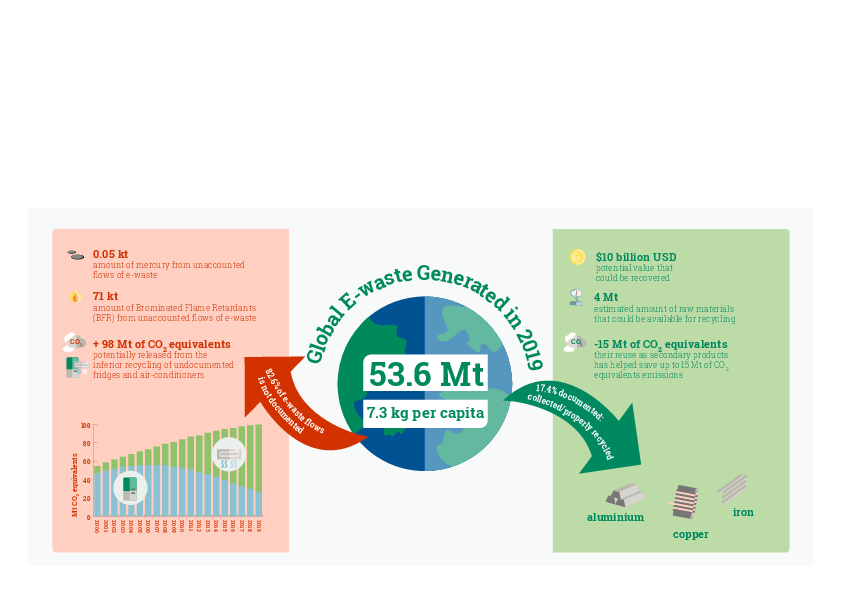
\includegraphics[width=0.9\textwidth]{Sections/Figs/Waste/EWaste-1.png}
    \caption{The generation of global E-waste in 2019. About 83\% of E-waste goes undocumented highlighting the importance of its re-use and recycling. Figure taken from Ref.~\cite{EWaste}.\label{fig:ewaste}}
\end{figure}

The topic of use of materials is also part of Section~\ref{sec:Technology}.

%%%%%

\begin{bestpractice}[Re-purposing shielding blocks\label{bp:HERAShieldingBlocks}]{Re-purposing shielding blocks}
Initially, the heavy concrete blocks in the HERA halls had served
as protection against radiation. Five hundred of these discarded shielding blocks were stored for years without being used on the DESY campus in Hamburg, Germany. 6000 tonnes of heavy concrete were shredded in 2020. The concrete rubble has become a new building material and is already being used for campus renovations~\cite{DESYsustainableReport2022}.
\end{bestpractice}

\subsubsection{Plastic Waste}
Plastic is a versatile product, efficient, cheap, stable, and infinitely moldable.  Its unique properties have resulted in our increasing reliance on it over decades, making it very hard to live without. 

GHG emissions from production, use and disposal of conventional (fossil-fuel-based) plastics is significant, and growing.  It is expected to increase to $\sim$2.1 \tCdOe\ per capita by 2040, accounting for almost 20\% of the global carbon budget~\cite{UNPollutionSolution}.  Under 10\% of plastic waste produced to date has been recycled, with the remainder being dumped or incinerated~\cite{UNPollutionSolution}.  This plastic waste contaminates the natural environment.  It is slow to degrade (`biodegradable' plastics included), releasing potentially harmful chemicals into the environment in the process, eventually breaking down to micro- and nano-plastic particles that wind up in the food chain.  Microplastics are also found in waste water, due to washing of synthetic textiles, and in cosmetic and personal care products~\cite{Microplastics}.  The health impacts of ingested plastic waste are not yet completely understood, but they are known to alter metabolic pathways and hormone signalling in animals.

A simple ban on single-use plastics, and plastics that are not at least 99\% recyclable would greatly limit microplastic pollution. 

\subsubsection{Conference Waste\label{sec:ConferenceWaste}}

The amount of waste generated at conferences could be significantly reduced by \eg keeping conference gifts digital (e-vouchers/discounts for local restaurants or activities) or replacing printed timetables and welcome packs with a well-designed conference app, see, \eg Whova\cite{Whova}.    Sustainable stationery could be distributed on a need-only basis, and banners, posters and nametags could be made plastic-free and reusable.  For waste-minimising initiatives implemented at the plastic-free 2019 conference of the Australian Marine Society, see~\bpref{bp:PlasticFreeConf}.  For sustainability concerns in conference catering see Section~\ref{sec:CateringTableware}


\begin{bestpractice}[Plastic-free 2019 conference of the Australian Marine Sciences Association\\
{\footnotesize Taken from Ref.~\cite{PlasticFreeConf}}\label{bp:PlasticFreeConf}]{Plastic-free 2019 conference of the Australian Marine Sciences Association}%
    In response to the growing problem of plastic pollution, the Australian Marine Sciences Association undertook to make their 2019 conference 100\% plastic free. Concrete measures they implemented for their roughly 600 delegates included:
    \begin{itemize}
        \item plastic-free cardboard name badges with bamboo lanyards and metal clips
        \item fabric tote bags give-aways with conference logo
        \item no printed envelopes for registration packs, no printed conference abstracts
        \item any printing necessary was done on sustainably-sourced paper, using a solar-powered printer
        \item sustainably-sourced pencils instead of pens, with sharpening stations provided
        \item no packaged sweets
        \item delegates were asked to bring reusable water bottles, or pre-register to buy them at the conference
        \item water jugs with glassware provided at back of each presentation room
        \item reusable, washable plates, cups silverware and glassware for all meal and coffee breaks
        \item vegetarian catering for tea breaks
    \end{itemize}
    These measures were implemented without affecting the budget, although some solutions reportedly took a fair amount of planning and forethought, and clear communication with the event organizer and providers.
\end{bestpractice}

\subsubsection{Catering Tableware}
\label{sec:CateringTableware}
A life-cycle analysis by the UN Environment Programme concludes that “reusable tableware consistently outperforms single-use tableware in all the studies and across all environmental impact categories (with water use being the exception, because of washing). This type of analysis takes into account all the variables that affect the environmental impact of a product, from manufacturing to end-of-life treatment. The case for reusable tableware is strengthened in countries where renewable energy makes up a high proportion of the grid mix and where end-of-life treatment options are not well developed”~\cite{UNEP2021}. 

In outdoor or remote environments or ‘pop-up’ events with no fixed catering facilities, where reusable tableware is impractical, single-use biodegradable tableware is preferable to other single-use tableware if it is industrially composted mixed in with food waste~\cite{UNEP2021}.\footnote{Industrial composting of household food waste is currently not the norm in most geographical locations within the USA~\cite{EPAWasteFoodMgmt}, and many existing industrial composters do not accept biodegradable plastic waste~\cite{BioplasticsAtIndustrialSites}.} 

Unlike emissions due to reusables, which are dominated by their use phase due to repeated washing, the  main impact of biodegradable tableware is due to its production. For conventional plastic, a significant role is also played by end-of-life management.  Quantitative analysis of their relative emissions is thus strongly dependent on assumptions about manufacture and disposal, including the material demand.  On the practical side, to minimise this impact when planning conference catering one should always choose the lightest-weight disposable tableware fit for purpose, preferably manufactured in a country with a significant proportion of renewables in its energy and electricity mix.  For a comparison of emissions due to different choices of catering tableware see~\csref{cs:conferencetableware}.

\begin{casestudy}[Comparing tableware for pop-up catering\label{cs:conferencetableware}]{Comparing tableware for pop-up catering}%
    Quantifying the environmental impact of single-use tableware is not simply a matter of quantifying its GHG emissions, as it has a significant impact across all environmental factors, including acidification, eutrophication, human health, land use and water depletion.  For the purposes of this case study, however, we will focus on its climate impact as the most urgent issue facing us today, and the one with the most reliable and robust indicators for decision making.

    We will consider for benchmarking purposes a large-scale conference with 1,000 attendees and informal lunchtime catering (\ie with no dishwashing capability), and compare the life-cycle emissions due to tableware made from conventional plastics, which are disposed of by a combination of incineration and landfill according to the European average (presumed food remnants making them unsuitable for recycling), and from biodegradable bioplastics, which are industrially composted along with the food remnants.

    We assume each set of tableware consists of a dinner plate and cup, a knife and fork, and a paper napkin and tray mat, all manufactured to the same size and thickness, but with possible differences in weight due to their respective material densities.  A full list of assumptions and details of the analysis can be found in the original article~\cite{Fieschi2018}.   

    The total emissions for 1,000 sets of conventional polystyrene tableware is 221 kg \CdOe, as compared with 109 kg \CdOe\ for the biodegradable bioplastic tableware, a saving of 112~kg \CdOe, around the emissions of a flight from Paris to Geneva.  Note that much of the comparative advantage of the bioplastics comes from their end-of-life treatment; their production is significantly more resource-intensive than conventional plastic tableware.  

    It is difficult to compare these figures to those for reusable tableware, since reliable, peer-reviewed studies that allow quantitative comparison between all three types of tableware are hard to come by.  For the purposes of comparison, however, we include here the emissions cost of 1,000 dishes and cups from a 2015 study by Italian plastics company Pro.mo~\cite{PROMO2015}.  They put the total emissions due to reusables at 26 kg \CdOe, with the emissions due to conventional plastic dishes and cups (polypropylene in this case) at 79 kg \CdOe.\footnote{We do not quote their estimate for bioplastics, since they do not consider the composting of bioplastics, but rather assume they are disposed of by incineration and landfill, in a similar way to conventional plastics.}

    Note that these figures are specific to the electricity and energy mix of the European market, which has a large impact on the dominant emissions in all cases: for production in the case of bioplastics, production and incineration for conventional plastics, and washing for reusables. 

\end{casestudy}

\end{document}